\documentclass[english]{article}
\usepackage[T1]{fontenc}
\usepackage[utf8]{luainputenc}
\usepackage{array}
\usepackage{float}
\usepackage{multirow}
\usepackage{amsmath}
\usepackage{graphicx}
\PassOptionsToPackage{normalem}{ulem}
\usepackage{ulem}

\makeatletter

\providecommand{\tabularnewline}{\\}

\usepackage{inputenc}
\usepackage{authblk}
\author[1,2]{Daniel Schlauch} 
\author[2,3]{Kimberly Glass}
\author[2]{Craig P. Hersh}
\author[2,4]{Edwin K. Silverman}
\author[1,3]{John Quackenbush}
\affil[1]{Department of Biostatistics and Computational Biology, Dana-Farber Cancer Institute and Department of Biostatistics, Harvard TH Chan School of Public Health, Boston, MA 02115}
\affil[2]{Channing Division of Network Medicine, Brigham and Women's Hospital, Boston, MA 02115}
\affil[3]{Department of Medicine, Harvard Medical School, Boston, MA 02115}
\affil[4]{Pulmonary and Critical Care Division, Brigham and Women's Hospital and Harvard Medical School, Boston, USA}

\@ifundefined{showcaptionsetup}{}{%
 \PassOptionsToPackage{caption=false}{subfig}}
\usepackage{subfig}
\makeatother

\usepackage{babel}
\begin{document}

\title{\textbf{Supplementary Materials for} \\
Estimating Drivers Cell State Transitions using Gene Regulatory Network
Models}

\maketitle

\part*{This PDF file includes:}
\begin{itemize}
\item Materials and Methods 
\item Supplementary Text 
\item Figs. S1 to S6
\item Tables S1, S2 
\end{itemize}
\renewcommand{\figurename}{Supplemental Figure}
\renewcommand{\tablename}{Supplemental Table}

\newpage{}


\section*{Materials and Methods }


\subsection*{\uline{Data Collection and Generation}}

Gene expression data from ECLIPSE, COPDGene, LGRC, and LTCOPD... {[}Kimbie
description{]}

Regulatory priors were created by using position weight matrices for
205 transcription factor motifs obtained from JASPAR 2014 http://jaspar2014.genereg.net/,
\cite{mathelier2013jaspar} and running Haystack\cite{pinello2014analysis}
to scan the hg19 genome for occurrences of these motifs. Sequences
were identified as hits for a transcription factor if they satisfied
the significance threshold of $p<10^{-5}$. We then linked motifs
to genes under the guidelines that a motifs is a possible transcription
factor binding sites for a particular gene if that motif is located
within 750 base pairs downstream or within 250 base pairs upstream
of a gene's promoter. We applied HOMER (http://homer.salk.edu/homer/ngs/index.html)
\cite{heinz2010simple} to identify motifs that met this criteria. 

Next, for each study, we identified transcription factors for which
we had gene expression data, removing those regulatory edges that
lacked corresponding expression values. Consequently, our motif prior
consisted of 164, 164, 148, and 145 transcription factors in ECLIPSE,
COPDGene, LGRC, and LTCOPD, respectively. MONSTER was run separately
on each of these studies. Comparisons of differential transcription
factor involvement across studies were performed on the 143 transcription
factors which were common to all four studies (Figure 3).


\subsection*{\uline{Common network inference methods do not produce reproducible
results in COPD}}

We evaluated the standard tools for COPD case-control studies at the
network level by observing the agreement in differential network inference
(NI) across studies. We utilizing the four studies - ECLIPSE, COPDGene,
LGRC, and LTCOPD. Our goal was to determine the ability of commonly
used NI methods to find reproducible results across studies. We tested
the methods Algorithm for the Reconstruction of Gene Regulatory Networks
(ARACNE), Context Likelihood of Relatedness (CLR), and Weighted Gene
Correlation Network Analysis (WGCNA). We computed differential edge-weights
across cases and controls using each of the NI methods. Next, we plotted
the differential edge-weights for each pairwise combination of studies
{[}\ref{Supplement NI edgeweight plots}{]}. We found no meaningful
correlation for edge-weight differences between \emph{any} two studies
using \emph{any} of the three methods. 

\begin{figure}[H]
\textbf{A}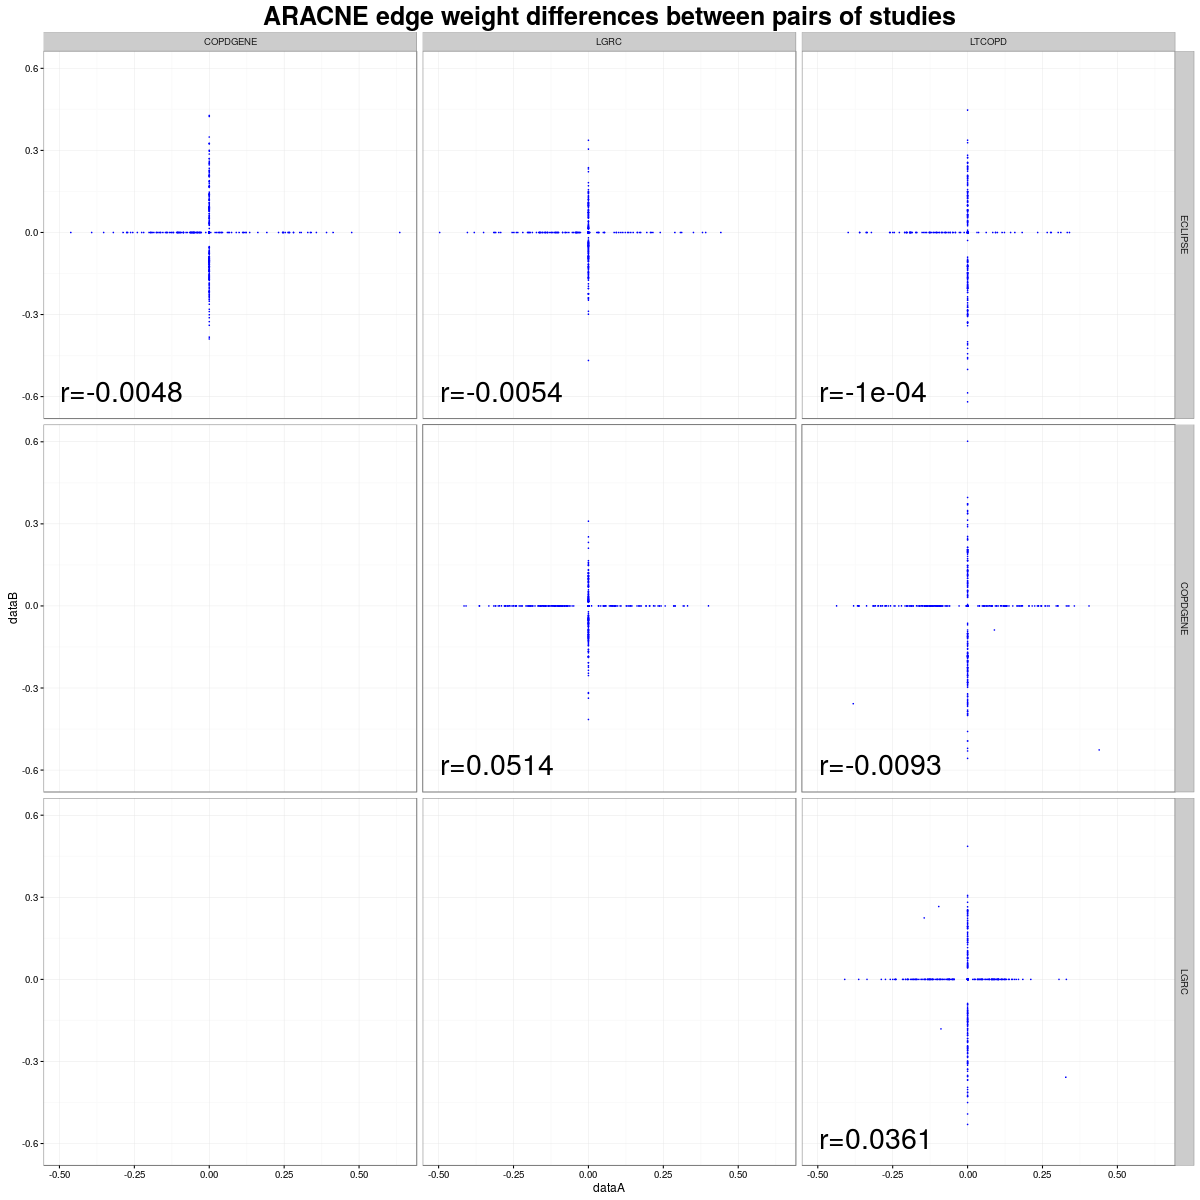
\includegraphics[width=0.45\columnwidth]{figures/all_studies_ARACNE_edgeweight_difference_comparison}\textbf{B}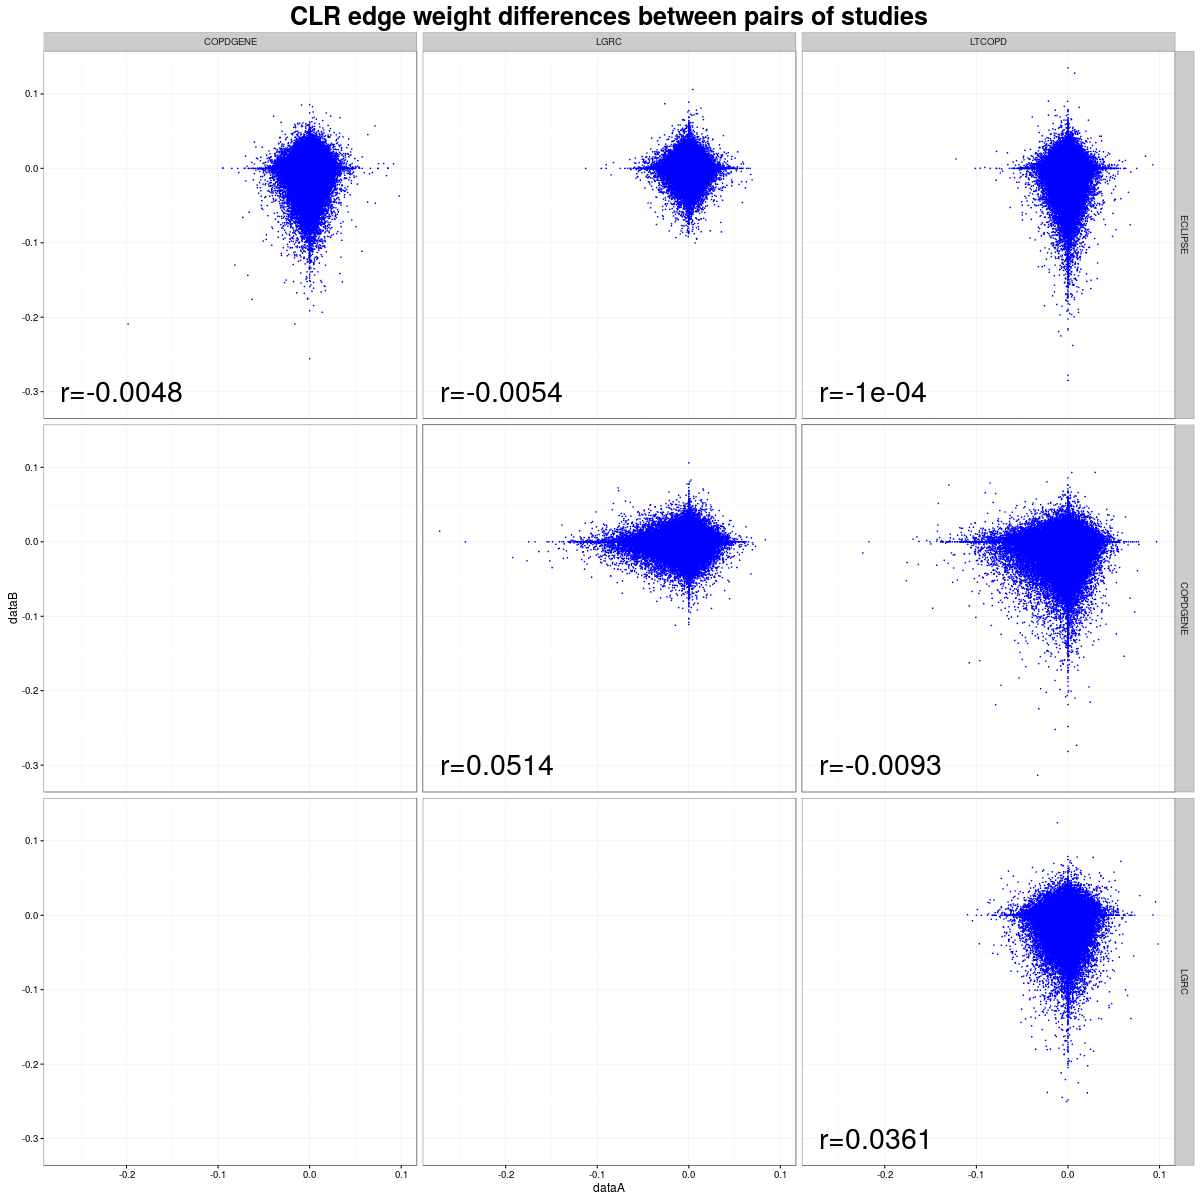
\includegraphics[width=0.45\columnwidth]{figures/all_studies_CLR_edgeweight_difference_comparison}

\textbf{C}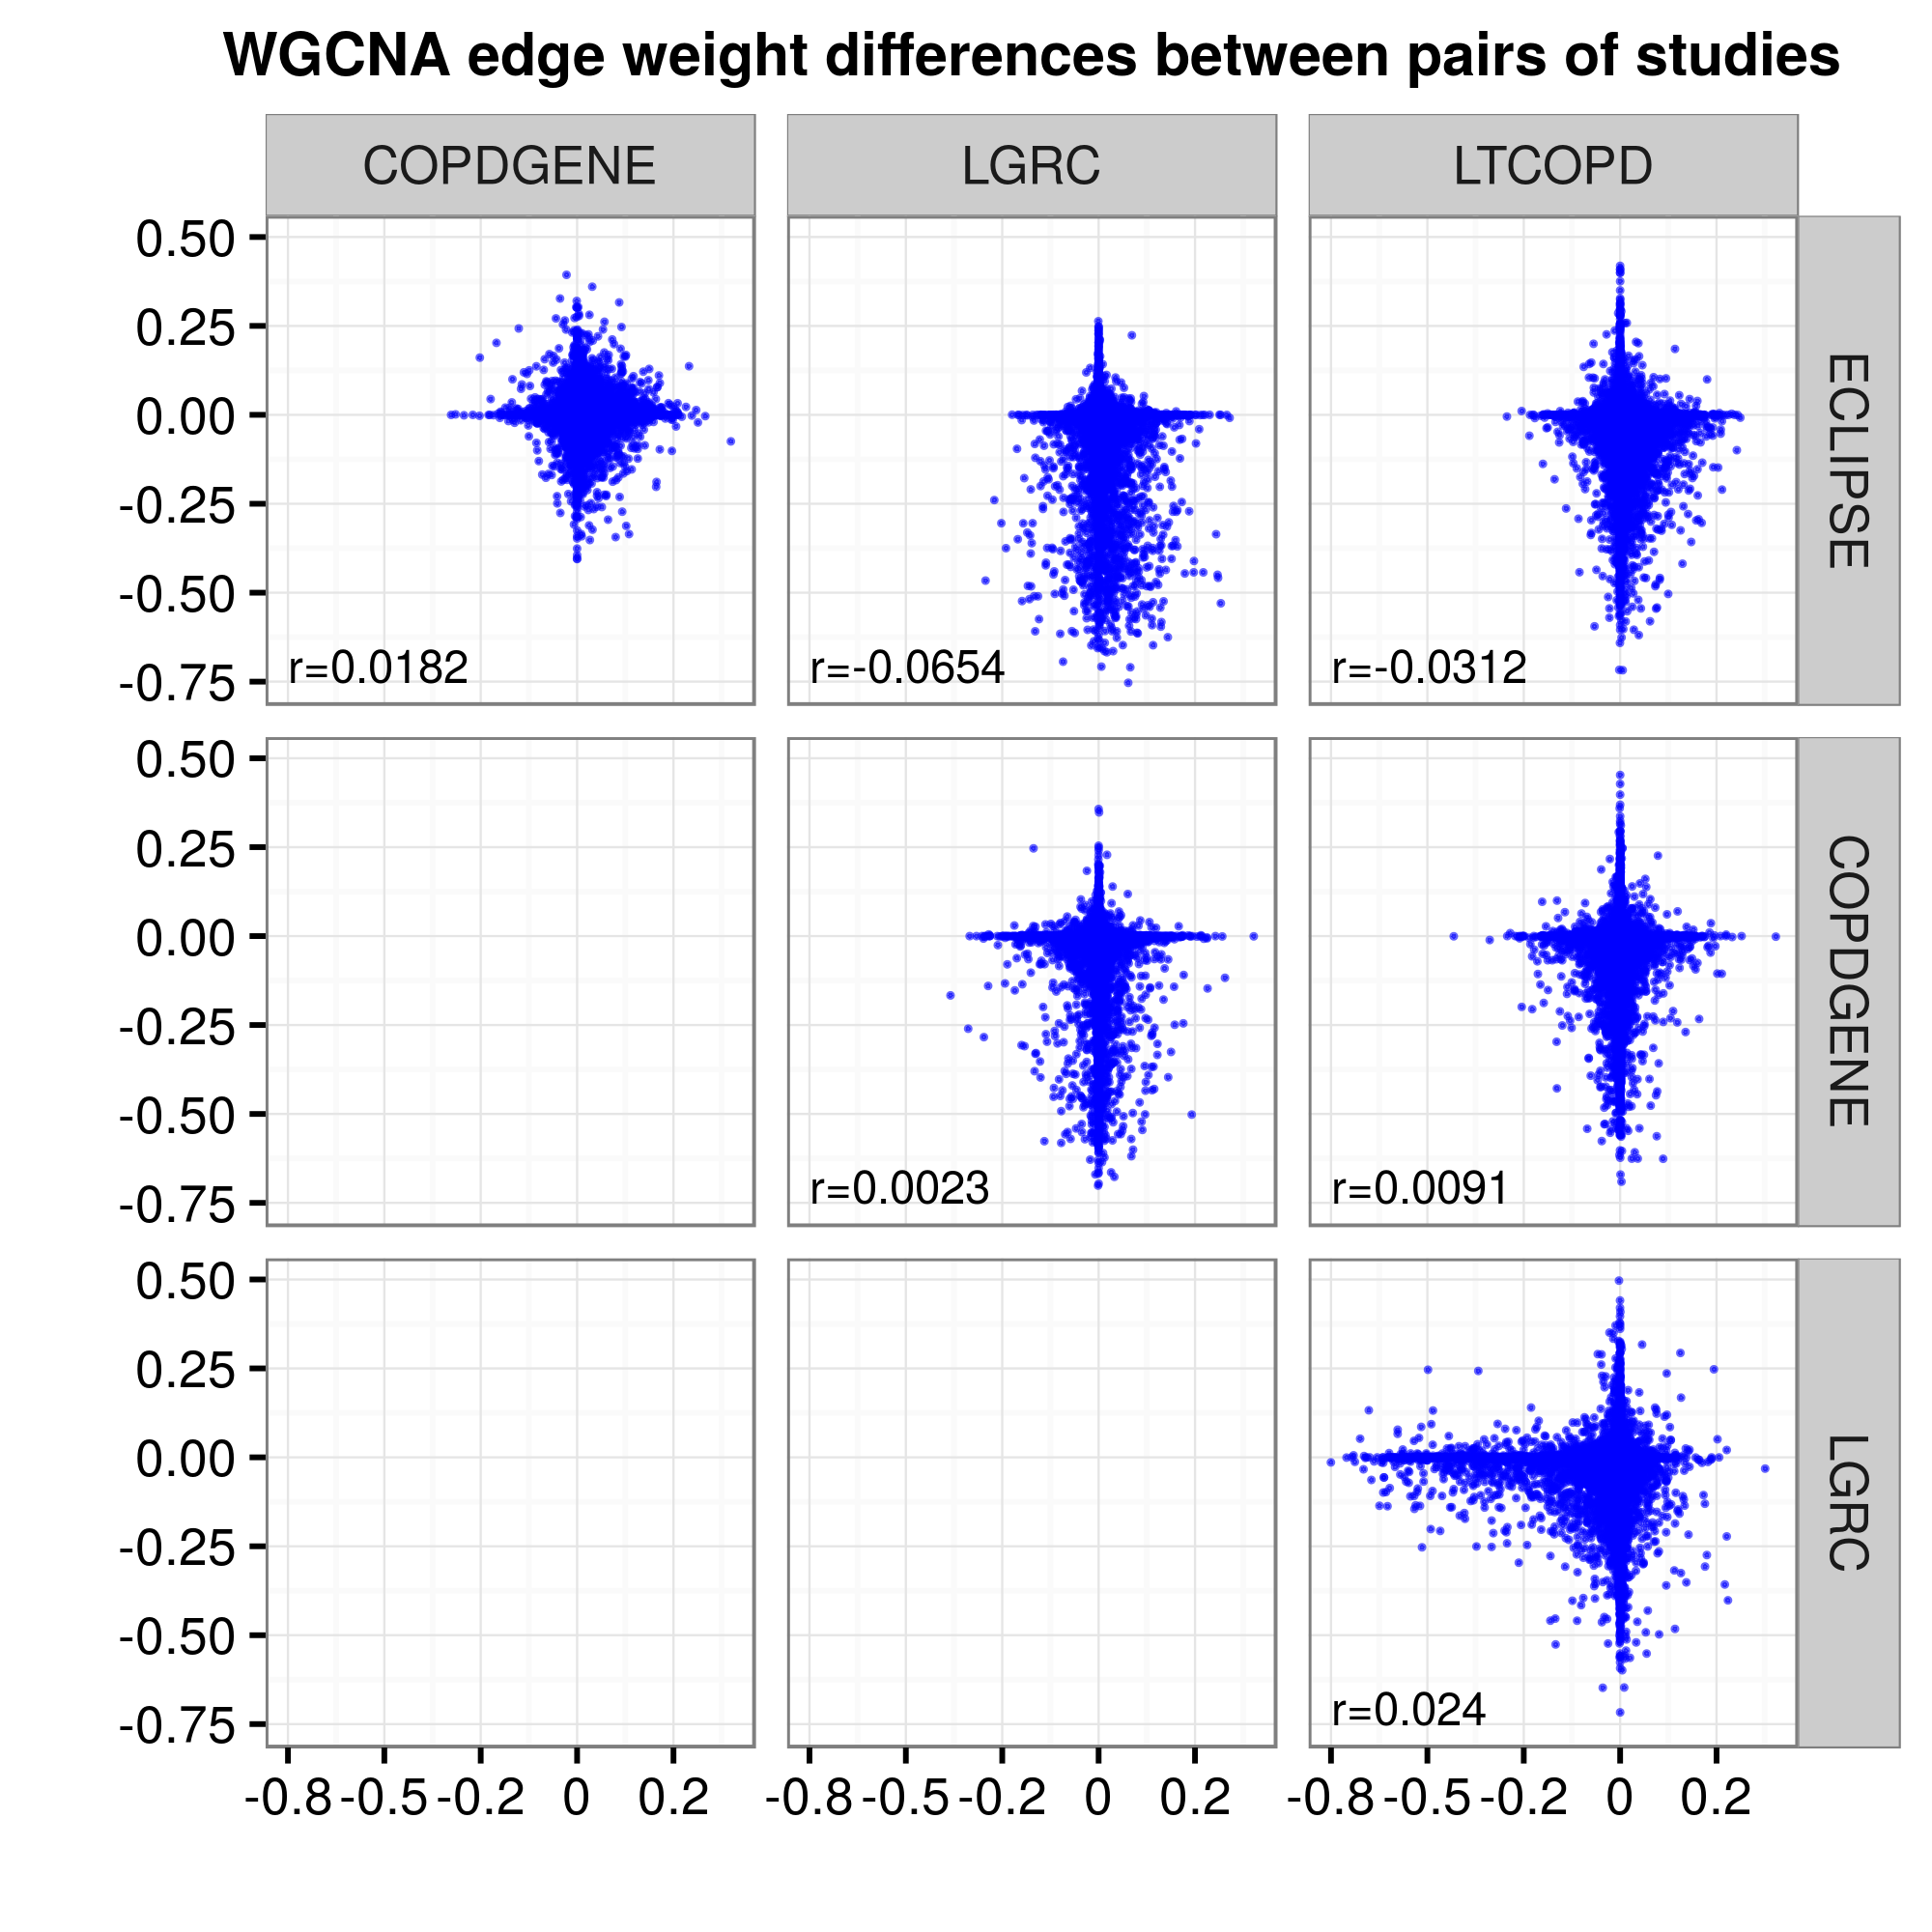
\includegraphics[width=0.45\columnwidth]{figures/all_studies_WGCNA_edgeweight_difference_comparison}\textbf{D}\includegraphics[width=0.45\columnwidth]{figures/all_studies_MONSTER_edgeweight_difference_comparison}\caption{\textbf{edge-weight differences between cases and controls do not
correlate across studies.} Using three commonly used network inference
methods from gene expression data, network inference was performed
separately on cases and controls. Here, the case-control difference
is compared across four independent studies of COPD. The methods tested
were \textbf{A} Algorithm for the Reconstruction of Gene Regulatory
Networks (ARACNE), \textbf{B} Context Likelihood of Relatedness (CLR),
\textbf{C} Weighted Gene Correlation Network Analysis (WGCNA), and
\textbf{D} MONSTER. No detectable agreement between studies exist
were found, regardless of network inference method or tissue type.}
\label{Supplement NI edgeweight plots}
\end{figure}


We conclude that identifying differences in COPD case-control studies
using existing methods for NI do not generate reproducible results.


\subsection*{\uline{Inferring Gene Regulatory Networks}}

In 2013, we described PANDA~\cite{glass2013passing}, a method~\cite{olsen2014inference}
for estimating gene regulatory networks that uses “message passing” ~\cite{frey2007clustering}
to integrate multiple types of genomic data. PANDA begins with a prior
regulatory network based on mapping transcription factor motifs to
a reference genome and integrates other sources of data, such as protein-protein
interaction and gene expression profiles, to estimate individual sample
networks. While PANDA has proven to be very useful in a number of
applications~\cite{lao2015genome,glass2015network,glass2014sexually},
its iterative approach to edge-weight optimization limits its utility
in situations requiring a large number of network bootstrap estimations.
To address this limitation, we developed an approach which considers
the available evidence of an edge for each possible TF-gene pair.
This evidence can be divided into two components, referred to here
as direct and indirect. Consider the edge between a TF and a gene,
referred to here as $TF_{i}$ and $g_{j}$, respectively. The direct
evidence, $d_{i,j}$, consists of the squared conditional correlation
of the $g_{i}$ and $g_{j}$ given all other regulators of $g_{i}$.
Where $g_{i}$ is the gene which encodes $TF_{i}$ 
\[
d_{i,j}=cor\left(g_{i},g_{j}|\left\{ g_{k,-j}:k\ne j,k\in\mathbf{TF}\right\} \right)^{2}
\]
 Naturally, the use of direct evidence inadequately captures regulatory
relationships due to the impacts of technical noise and numerous biological
external factors such as stable or transient protein-protein interactions,
post-translational modifications, etc. which may confound or modify
a regulatory effect. These sources of confounding and variability
in the expression pattern of a gene coding a TF may obscure the effects
it has on all of its target genes. Therefore it is of value if we
can complement our estimate of the likelihood of a regulatory mechanism
by aggregating the information from the gene expression patterns of
all suspected targets of transcription factors. PANDA achieves its
superior performance in part by convergence towards “agreement”, whereby
large collections of gene expression patterns must agree with the
proposed regulatory structure in order to claim an interaction. Similarly,
we look for agreement between the gene expression patterns of large
sets of co-targeted genes. We refer to this feature as indirect evidence
and can achieve this by again utilizing our set of regulatory priors.
In this portion of the analysis we suspend the recognition of a TF
as a member of the gene list and instead consider each of the $m$
TFs to be binary classifications across the entire gene list. Class
labels are determined by the presence or absence of a sequence binding
motif for that TF in the vicinity of the gene.

The indirect evidence between the two nodes, $\theta_{i,j}$, represents
the fitted probability that $g_{i}$ belongs to the class of genes
targeted by $TF_{j}$. $g_{i}$ is considered to be a new observation
placed into the \emph{n}-dimensional space separated by transcription
factor targets and non-targets. To divide up the space, we use a logistic
regression on the gene expression data with outcome taken to be the
existence or non-existence of a known sequence motif for $TF_{j}$
upstream of $g_{i}$. 
\[
logit\left(E\left[M_{j}\right]\right)=\beta_{0}+\beta_{1}g_{\left(1\right)}+\dots+\beta_{N}g_{\left(N\right)}
\]
where the response $M_{j}$ is a binary vector of length $n$ indicating
the of the presence of a sequence motif for transcription factor $j$
in the vicinity of each of the $n$ genes. And where $g_{\left(k\right)}$
is a vector of length $n$ specifying the gene expression for sample
$k$ over $n$ genes. 

For some TF-gene pair, the fitted values for each $TF_{j}-g_{i}$
pair define the ``indirect'' evidence $\theta_{j,i}$.
\[
\hat{\theta}_{j,i}=\frac{1}{1+e^{\beta_{0}+\beta_{1}g_{i,\left(1\right)}+\dots+\beta_{k}g_{i,\left(k\right)}}}
\]


By scoring each gene according to the strength of indirect evidence
for a regulatory response to each of the TFs, we can combine this
with the direct evidence of regulation (squared conditional correlation
of expression for $g_{i}$ and $TF_{j}$). The appropriate manner
in which to combine direct and indirect evidence remains an open question.
Though both measures are bounded by {[}0,1{]} their interpretation
is quite different. The direct evidence can be considered in terms
of it's conditional gene expression $R^{2}$ between nodes, while
the indirect evidence is interpreted as a probability. We use a non-parametric
approach to combine evidence. The targets of each TF are then ranked
and combined as a weighted sum, $w_{i}=\left(1-\alpha\right)\left[rank\left(d_{i}\right)\right]+\alpha\left[rank\left(e_{i}\right)\right]$,$i\in\left\{ 1,\dots,n\right\} $.
Our choice of the weight, $\alpha$, here is based on empirical evaluation,
and perhaps not surprisingly, is loosely correlated with organism
complexity. In validation sets from Yeast, the optimal alpha was observed
near $\alpha=.9$ while simpler E. coli datasets saw an optimal value
of $\alpha=.6$ and an in silico dataset, optimal $\alpha$ was achieved
at $\alpha<.5$ This naturally reflects the fact that the increased
complexity of the network necessitates the use of larger scale agreement
between genes, rather than a reliance on pairwise correlations between
potentially noisier and more complex expression patterns. 


\subsection*{\uline{Network edges are recovered in In Silico, E. coli and Yeast
(}\emph{\uline{Saccharomyces cerevisiae}}\uline{)}}

A common challenge in gene regulatory network inference is the difficulty
of validating identified networks against a known, reliable gold standard.
A number of validation methods have been used for in vivo samples,
including ChIP-seq, ChIP-chip. Knockdowns have also been used in cell
lines and have been shown to be effective at predicting in vivo responses
\cite{olsen2014inference}. Additionally, in silico methods have been
used which simulate gene expression datasets based on a predefined
set of regulatory mechanisms.

To test our methods, we used four test datasets of increasing biological
complexity- (1) in silico, (2) E. coli, and (3) Yeast with simulated
motif priors and (4) Yeast with biological motif priors. Data from
(4) was collected from \emph{Saccharomyces cerevisiae} with TF knock-out
and stress conditions \cite{harbison2004transcriptional}. Data from
the first three sources was obtained from the publicly available DREAM5
challenge\cite{marbach2012wisdom}. This challenge asked contestants
to infer gene networks from expression data alone, using a gold standard
for evalution. Instead, we started with the gold standard and swapped
a number of edges to create the type I and type II error rates consistent
with Yeast motif priors and evaluated the performance of MONSTER to
refine its predictions of the true gold standard. The estimated edges
in MONSTER utilizing the gene expression data were demonstrated to
be superior to those of the edge prior alone.

\begin{figure}
\textbf{A}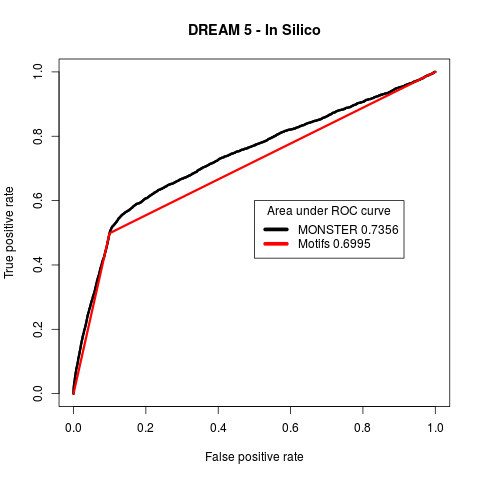
\includegraphics[width=0.4\columnwidth]{figures/DREAM5a_all}\textbf{B}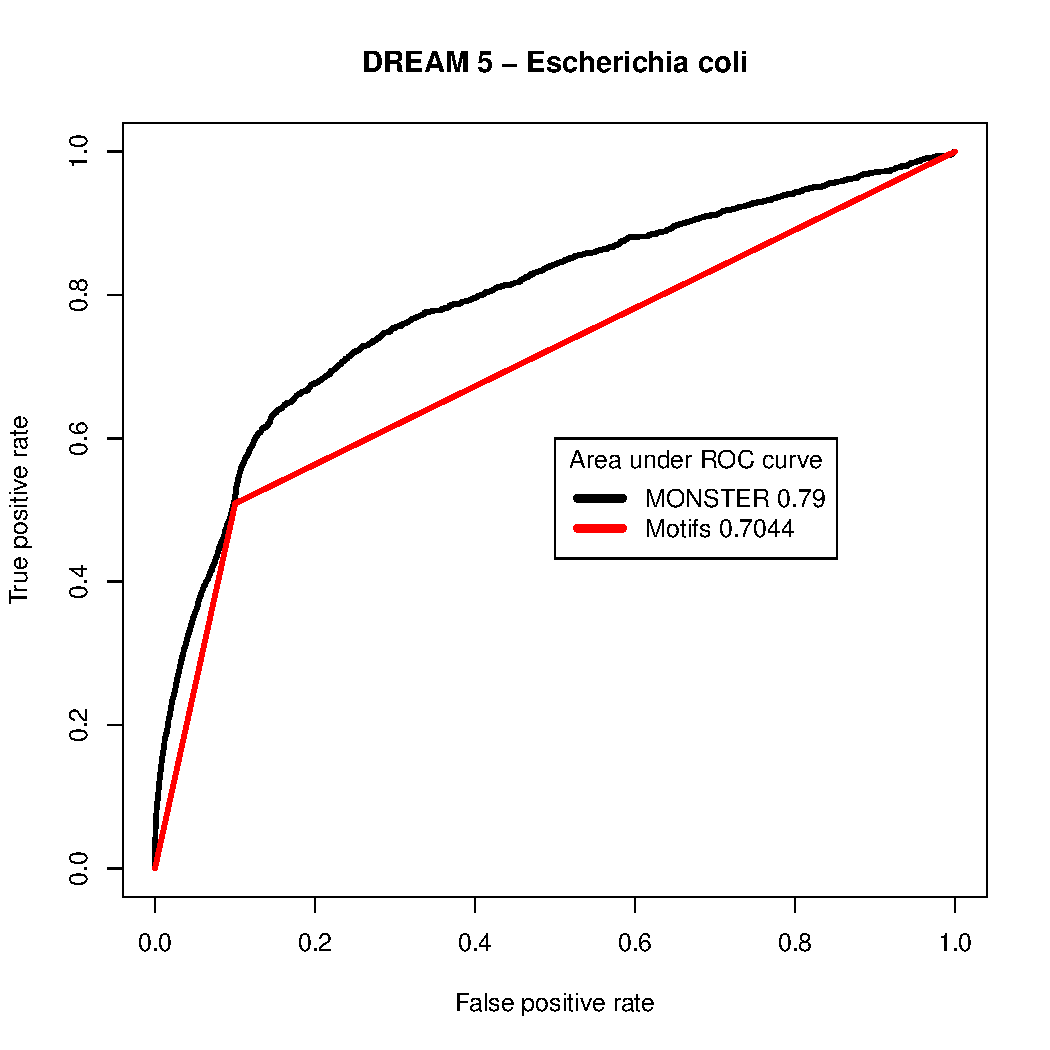
\includegraphics[width=0.4\columnwidth]{figures/DREAM5c_all}

\textbf{C}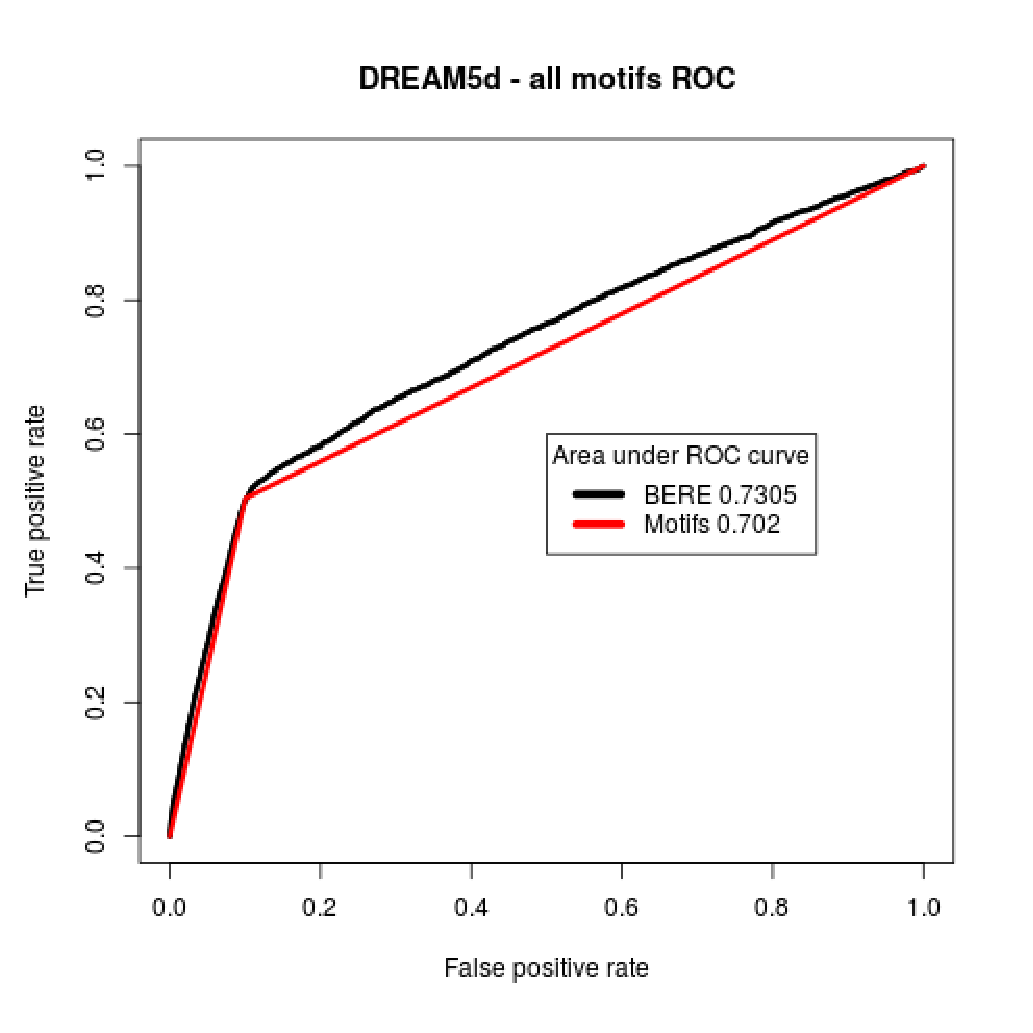
\includegraphics[width=0.4\columnwidth]{figures/DREAM5d_all}\textbf{D}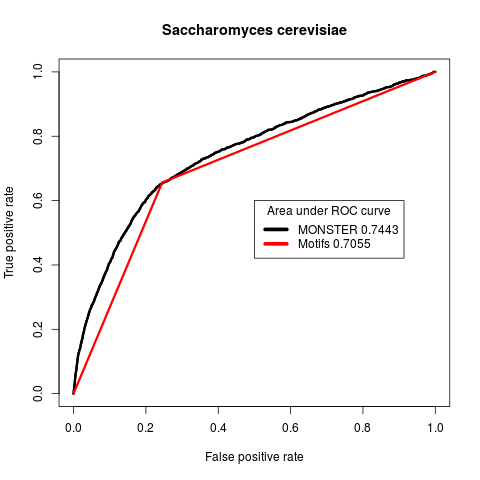
\includegraphics[width=0.4\columnwidth]{figures/Yeast_all}\caption{Receiver-Operator Characteristic curves for three DREAM 5 datasets
(A) in silico, (B) E. coli, (C) Saccharomyces cerevisiae, and an (D)independent
Saccharomyces cerevisiae dataset. The initial prior network in each
of the DREAM 5 datasets was taken from the gold standard, with error
introduced (both type I and type II) bringing the area under the ROC
curve to $\approx0.70$. In the Saccharomyces cerevisiae, sequence
motifs were used as the prior with CHiP-chip binding sites used as
the gold standard. In each of these tests, measureable improvement
in performance of MONSTER's network inference method over the prior
network is observed.}
\end{figure}



\subsection*{\uline{Computation of MONSTER’s transition matrix}}

A primary purpose of reconstructing GRNs is the understanding of the
biological mechanisms which characterize disease. Identifying differential
TF targeting may suggest a therapeutic target, uncover a disease substructure
or identify biomarkers for early detection. However, significant limitations
exist with respect to generating reliable context-specific GRNs. Substantial
advances have been made in this area with algorithms like SEREND and
PANDA, but these methods rely more heavily on the static sequence
motif data rather than gene expression data collected across groups,
such as in a case-control study. Both methods, along with MONSTER's
network inference approach, use gene expression data as a refinement
of the more accurate motif priors. It is therefore a side effect that
any GRN inference method that relies on motifs directly for edge-weight
calculation will be susceptible to having the bulk of its predictive
power stripped when making comparisons between networks. Consequently,
it is of critical importance to choose a network inference method
that uses the context-specific data to most accurately refine above
what information is gleaned from our static data.

The task of identifying meaningful network transitions then becomes
an evaluation of the relative refinement of edge-weights. Since the
majority of the predictive power for each edge is contained in the
motif contribution, we are left with relative edge-weight refinement
that have a low signal, high noise. In other words, we have a very
large number of individually unreliable edge-weights. In effort to
extract the maximum effect, we seek to combine the information contained
in each edge via a novel dimension reduction approach.

Consider two adjacency matrices, $\mathbf{A},\mathbf{B}$ representing
the two GRNs estimated from a case-control study. Each matrix has
dimensions $\left(p\times m\right)$ representing the set of $p$
genes targeted by $m$ TFs. We seek a matrix, $\mathbf{T}$, such
that 
\[
\mathbf{B}=\mathbf{AT}+\mathbf{E}
\]
Where $\mathbf{E}$ is our error matrix, which we want to minimize.
Intuitively, we may frame this as a set of $m$ independent regression
problems, where $m$ is the number of transcription factors and also
the column rank of $\mathbf{A},\mathbf{B},\mathbf{T}\,and\,\mathbf{E}$.
For a column in $\mathbf{B}$, $\mathbf{b}_{i}$, we note that a corresponding
column in $\mathbf{T}$, $\mathbf{\tau}_{i}$, represents the OLS
solution to
\[
E\left[\mathbf{b}_{i}\right]=\tau_{i1}\mathbf{a}_{1i}+\tau_{i2}\mathbf{a}_{2i}+\dots+\tau_{im}\mathbf{a}_{mi}
\]
or alternatively expressed 
\[
\left[\begin{array}{c}
\mathbf{b}_{i1}\\
\mathbf{b}_{i2}\\
\vdots\\
\mathbf{b}_{ip}
\end{array}\right]=\mathbf{\tau}_{1,i}\left[\begin{array}{c}
\mathbf{a}_{11}\\
\mathbf{a}_{21}\\
\vdots\\
\mathbf{a}_{p1}
\end{array}\right]+\mathbf{\tau}_{2,i}\left[\begin{array}{c}
\mathbf{a}_{12}\\
\mathbf{a}_{22}\\
\vdots\\
\mathbf{a}_{p2}
\end{array}\right]+\dots+\mathbf{\tau}_{p,i}\left[\begin{array}{c}
\mathbf{a}_{1p}\\
\mathbf{a}_{2p}\\
\vdots\\
\mathbf{a}_{pp}
\end{array}\right]+\left[\begin{array}{c}
e_{i1}\\
e_{i2}\\
\vdots\\
e_{ip}
\end{array}\right]
\]


where $E\left[e_{ij}\right]=0$ 

This can be solved with normal equations, 
\begin{eqnarray*}
\mathbf{\tau}_{i} & = & \left(\mathbf{A}^{T}\mathbf{A}\right)^{-1}\mathbf{A}^{T}\mathbf{b}_{i}\\
\mathbf{T} & = & \left[\tau_{1},\tau_{2},\dots,\tau_{m}\right]
\end{eqnarray*}
Which produces the least squares estimate. I.e. loss function $L\left(\mathbf{T}\right)=\sum_{gene=1}^{N}||\mathbf{B}_{gene}-\mathbf{A}_{gene}\mathbf{T}||^{2}$
is minimized. We further extend this method to include a penalty term\cite{tibshirani1996regression}.
An $L_{1}$ regularization is used by creating an identity penalty
model matrix for each column regression such that only the $k^{th}$
diagonal element is 0 and all other diagonals are 1. This gives priority
for the $k^{th}$ regression coefficient in the $k^{th}$ regression
model. 
\[
\mathbf{Q}_{i,j}=\begin{cases}
1 & for\,i=j\ne k\\
0 & elsewhere
\end{cases}
\]
This solution is obtained using the ``penalized'' library in R as
the minimization of the penalized squared loss function
\[
\sum_{i=1}^{p}\left(\mathbf{B}_{i,k}-\sum_{j=1}^{m}A_{i,j}\mathbf{T}_{j,k}\right)^{2}+\lambda\mathbf{\sqrt{\beta^{\prime}Q\beta}}
\]


This example illustrates a key feature of this method. Specifically,
that the transition matrix reduces the case-control network transformation
from a set of $2\times p\times m$ estimates to a set of $m\times m$
estimates that are easily interpreted. We can think of a column, $\tau_{i}$,
on the matrix $\mathbf{T}$ as containing the linear combination of
regulatory targets of $TF_{i}$ in $\mathbf{A}$ that best approximates
the regulatory targets of $TF_{i}$ in $\mathbf{B}$. As one would
expect, a large proportion of the matrix ``mass'' would be on the
diagonal for those TFs which do not change regulatory behavior between
case and control. It is therefore of interest to evaluate values off
of the diagonal as indications of a network transition.


\subsection*{\uline{Evaluating the Transition Matrix}}

Many mechanisms which may be differentially present, such as RNA degredation,
post-translational modification, protein-level interactions and epigenetic
alterations have the ability to impact downstream targeting without
impacting the expression level of the TF itself. It may be of particular
scientific or therapeutic interest to identify those TFs which have
undergone significant overall changes in behavior between controls
and cases. With that objective in mind, we express the statistic-
differential Transcription Factor Involvement (DTFI), as a measure
for quantifying this property. 
\[
s_{j}=\frac{\sum_{i=1}^{m}I\left(i\ne j\right)\tau_{i,j}^{2}}{\sum_{i=1}^{m}\tau_{i,j}^{2}}
\]
 DTFI can be loosely interpreted as the proportion of TF targeting
patterns which is explained by the targeting patterns of other available
TFs. This measure, a statistic on the interval $[0,1]$ seeks to elucidate
transitions which are systematic, informative, and non-arbitrary in
nature by capturing only the edge-weight signal for which there is
an attributable regulatory pattern. The distribution of this statistic
under the null has a mean and standard deviation which depend on the
motif structure. In particular, both mean and standard deviation are
increased for TFs which have fewer prior regulatory targets. From
a statistical perspective, TFs with relatively more targets are able
to generate more stable targeted expression patterns, which leads
to more consistent estimates in “agreement” algorithms such as PANDA.
From a biological perspective, increased motif presence may indicate
that the TFs are more likely to be ubiquitous housekeeping proteins
that do not meaningfully alter their involvement between cases and
controls. The dependence of the null distribution on the motif structure
is addressed via the following resampling procedure. 
\begin{enumerate}
\item Gene expression samples are randomly assigned to case and control
forming the null-case and null-control with group sizes preserved. 
\item GRNs are reconstructed for the null-case and null-control with the
same prior regulatory structure. 
\item The transition matrix algorithm is applied for the two null networks. 
\item The differential TFI is calculated for each TF. 
\item Repeat 1-4 1000 times. 
\end{enumerate}
\begin{figure}
\centering{}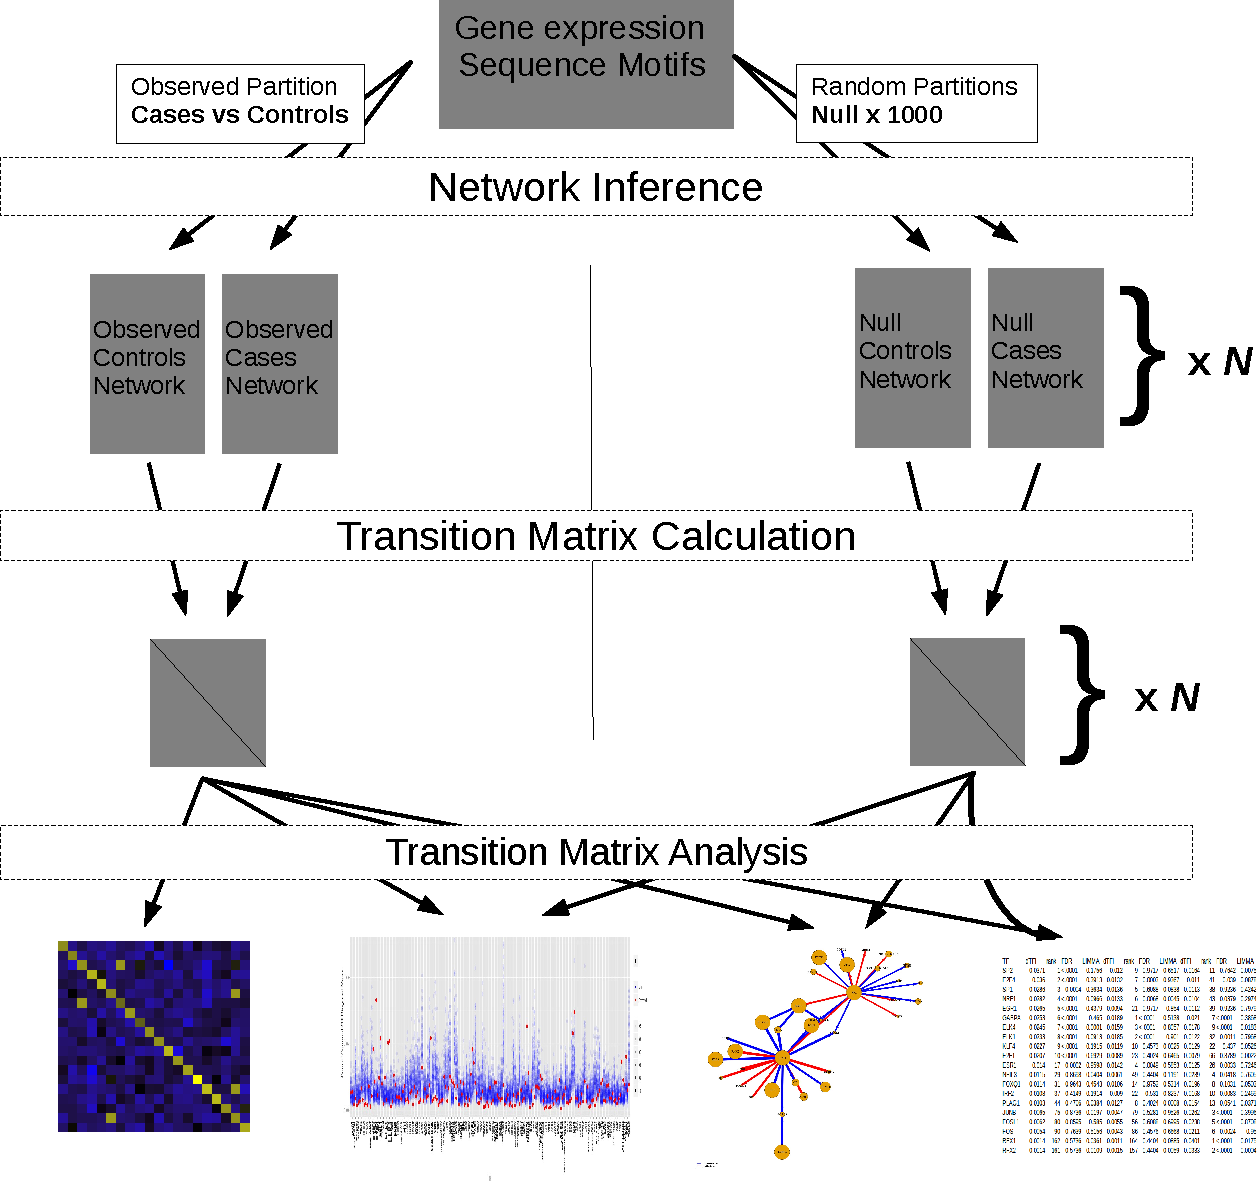
\includegraphics[width=0.8\columnwidth]{figures/workflow_diagram}\caption{\textbf{Overview of MONSTER analysis workflow.} (1) Network inference
is computed separately to subsets of the gene expression data including
the cases group, the controls group and 1000 permutations of the cases
and controls labels. (2) Transition matrix is estimated between the
cases and controls and each of the pair or permuted ``cases'' and
``controls''.}
\end{figure}



\subsection*{\uline{MONSTER significantly improves TF-TF edge estimation from
}\emph{\uline{in silico}}\uline{ gene expression data} }

To evaluate the ability of our method to recover edges between transcription
factors, we generated simulated gene expression data. We began by
generating a true controls adjacency matrix, $M_{0\left(p\times q\right)}$,
describing the weighted edges between $q$ transcription factors and
$p$ genes. A state transition was generated by sampling 100 TF-TF
pairs and adjusting the edge-weight at the corresponding point on
the true cases adjacency matrix, $M_{1\left(p\times q\right)}$. These
TF-TF pairs ultimately represent the edges that we seek to recover
and the size of the adjustments are the parameters of interest. We
sampled from a multivariate Gaussian distribution with the off-diagonal
of the variance-covariance matrix, $\Sigma$, defined as the $M_{0}M_{0}^{\prime}$.
Furthermore, we scaled the magnitude of the diagonal of $\Sigma$
to achieve the desired proportion of noise. We aimed for an area under
the curve of the receiver-operator characteristic of approximately
0.70 as this has reasonably been achieved in existing biological studies~\cite{glass2013passing}.
We note that the two simulated regulatory priors have AUC-ROC of .570
and .547, which feeds the MONSTER and PANDA algorithms with priors
which are substantially less predictive than sequence motif priors
commonly used for network inference methods.

This sampling represented our simulated control samples. The adjusted
adjacency matrix, $M_{1}$, was similarly used to generate simulated
expression data for the cases group. Next, we reconstructed the networks
from our expression data using a set of commonly used network inference
methods - Weighted Gene Correlation Network Analysis (WGCNA)~\cite{Langfelder2008WGCNA}~\cite{Langfelder2008FastR},
Topological Overlap Measure (TOM)~\cite{ravasz2002hierarchical},
Algorithm for the Reconstruction of Gene Regulatory Networks (ARACNE)~\cite{margolin2006aracne},
Context Likelihood of Relatedness (CLR)~\cite{faith2007large}, Passing
Attributes between Networks for Data Assimilation (PANDA)~\cite{glass2013passing}
and simple Pearson correlation (PC). 

We applied the transition matrix with default parameters on each case-control
pair of networks. For comparison, we estimated the difference from
case to control in edge-weights derived from the direct edge prediction
using each network inference method. The predictions for the TM approach
and the direct approach were evaluated by the area-under-the-curve
of the receiver-operator-characteristic (AUCROC) with the true transition
adjustments taken as the gold standard. For each of the network inference
methods tested, we found substantial improvement in the predicted
transitions over the direct network inference method. In many cases,
the edge-weight difference (column 2) was not statistically significant
for predicting transitions, but when the TM was applied (column 3)
a strong predictive signal appeared. In other cases, an existing signal
was observed using the direct approach, but was dramatically improved
with the application of the TM.

The intuition behind the improvement is simple. While the estimation
of a TF-TF edge is typically evaluated via some pairwise gene expression
pattern which may be rife with technical and biological noise, the
TM approach borrows information from all downstream targets in estimating
the relative change in relationship between the TFs. 

{\tiny

\begin{table}
\begin{tabular}{|cc||c|c|}
\multicolumn{4}{c}{AUC-ROC for edge-weight differences vs Transition Matrix using various
NI methods}\tabularnewline
\hline 
\multirow{2}{*}{\textbf{NI Method}} & \multirow{2}{*}{\textbf{Network AUC}} & \textbf{edge-weight } & \textbf{MONSTER}\tabularnewline
 &  & \textbf{differences} & \tabularnewline
\hline 
Pearson & .704 & .510 (p=.72) & .802 (p<.0001)\tabularnewline
\hline 
WGCNA(6) & .704 & .512 (p=.61) & .688 (p<.0001)\tabularnewline
\hline 
WGCNA(12) & .704 & .52 (p=.10) & .589 (p=.02)\tabularnewline
\hline 
ARACNE & .515 & .523 (p=.58) & .566 (p=.09)\tabularnewline
\hline 
CLR & .694 & .57 (p=.19) & .814 (p<.0001)\tabularnewline
\hline 
TOM & .703 & .51 (p=.62) & .689 (p<.0001)\tabularnewline
\hline 
PANDA{*} & .747 & .520 (p=.13) & .793 (p<.0001)\tabularnewline
\hline 
PANDA{*}{*} & .652 & .509 (p=.43)  & .66 (p<.0001) \tabularnewline
\hline 
\end{tabular}\caption{\textbf{Comparison of edge-weight difference to Transition Matrix
in simulated case-control gene expression}. Several network inference
methods were run on our \emph{in silico} case-control data. The overall
network area under the curve of the receiver-operator characteristic
(AUC-ROC) was performed for each method averaged across cases and
controls. For PANDA{*} and PANDA{*}{*}, which additionally utilizes
motif prior information, motif priors with AUC-ROC of .570 and .547
were used. The naive TF-TF transitions were calculated as the difference
in TF-TF edge-weight between cases and controls. The transition matrix
TF-TF transitions used the absolute transition matrix values. }
\end{table}


}


\subsection*{\uline{MONSTER finds significant protein-protein interaction}}

As noted above, there are numerous biological regulatory mechanisms
which may yield detectable transitions. Of particular interest are
those which are less readily detectable via conventional methods,
such as differential gene expression analysis. One mechanism studied
here involves one TF binding to another TF to promote, suppress or
alter one or both of their regulatory patterns. These multi-protein
interactions create combinatorial complexity that can explain much
of the variation in organism complexity which is unexplained by gene
expression alone~\cite{levine2003transcription}.

To test the ability to detect protein level interactions, we compared
our estimated transitions to a set of known protein-protein interactions
\cite{ravasi2010atlas}. This set contained 223 interactions between
our set of transcription factors, of which 39 were self-interacting
and were removed. We attempted to predict the remaining 184 interactions
between transcription factors using MONSTER. Of interest was the effectiveness
of identifying these interactions via the transition from one phenotypic
state to another. This is a challenging task for several reasons,
(1) protein-protein interaction is merely one of a myriad of detectable
transition mechanisms which MONSTER is designed to detect, (2) it
is reasonable to assume that only a small subset of the known PPI
are actually differentially present between cases and controls in
a particular study and (3) technological limitations in the active
field of proteomics cannot be expected to identify all interactions
with a reasonable degree of certainty.

We measured the ability to identify suspected interactions by running
MONSTER on the 84 smoker controls and the 136 COPD patients in the
ECLIPSE study. We used the absolute value of each element in the transition
matrix to serve as the predictor of PPI and computed the area under
the ROC curve. To identify the significance of AUC-ROC, we ran MONSTER
on 400 iterations of randomized phenotypic labels and computed the
AUC-ROC for each iteration. 

We achieved only an AUC-ROC score of $.548$ suggesting weak predictive
power of MONSTER for identifying known PPI in the ECLIPSE study, but
this result exceeded all randomized phenotype results and was significant
at $p<.0025$. This indicates that this weak, but significant result
was driven by the differentiation of COPD patients and smoker controls.
Notably, MONSTER was able to extract a small but significant protein
interaction signal from highly obfuscated data.

\begin{figure}
\subfloat[\textbf{ECLIPSE}]{\textbf{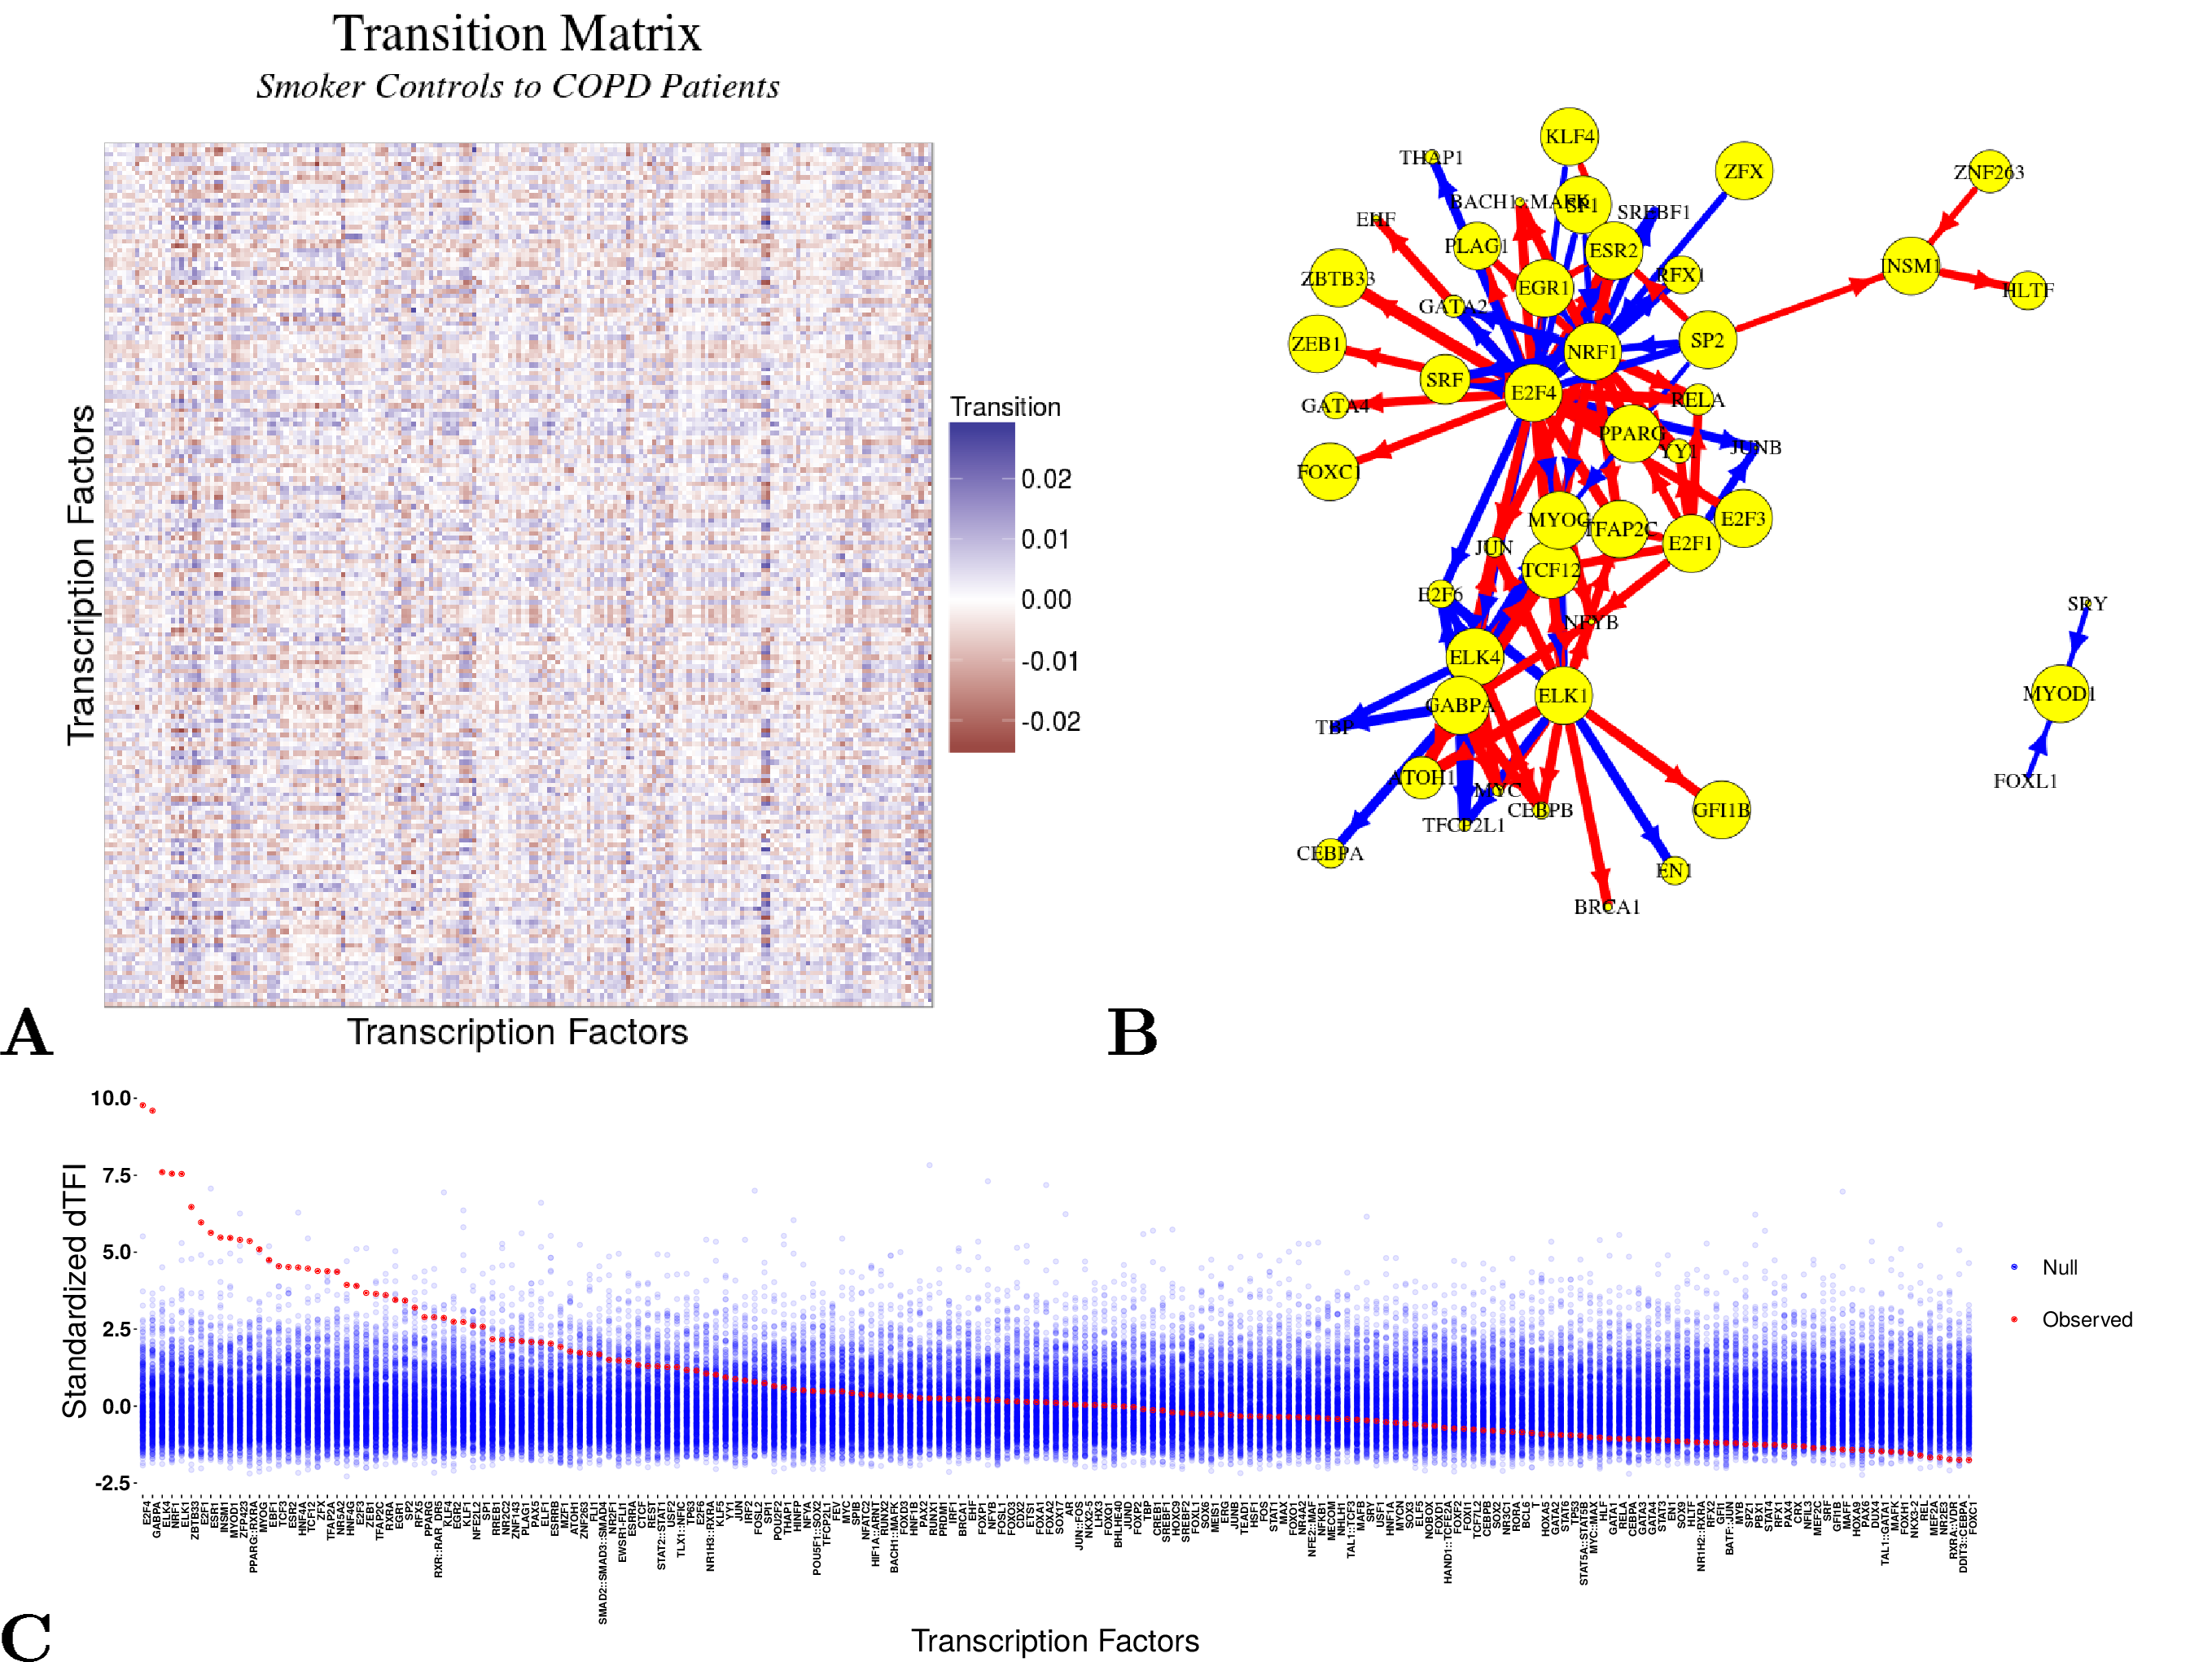
\includegraphics[width=0.49\columnwidth]{figures/figure2ECLIPSE}}}

\subfloat[\textbf{COPDGENE}]{\textbf{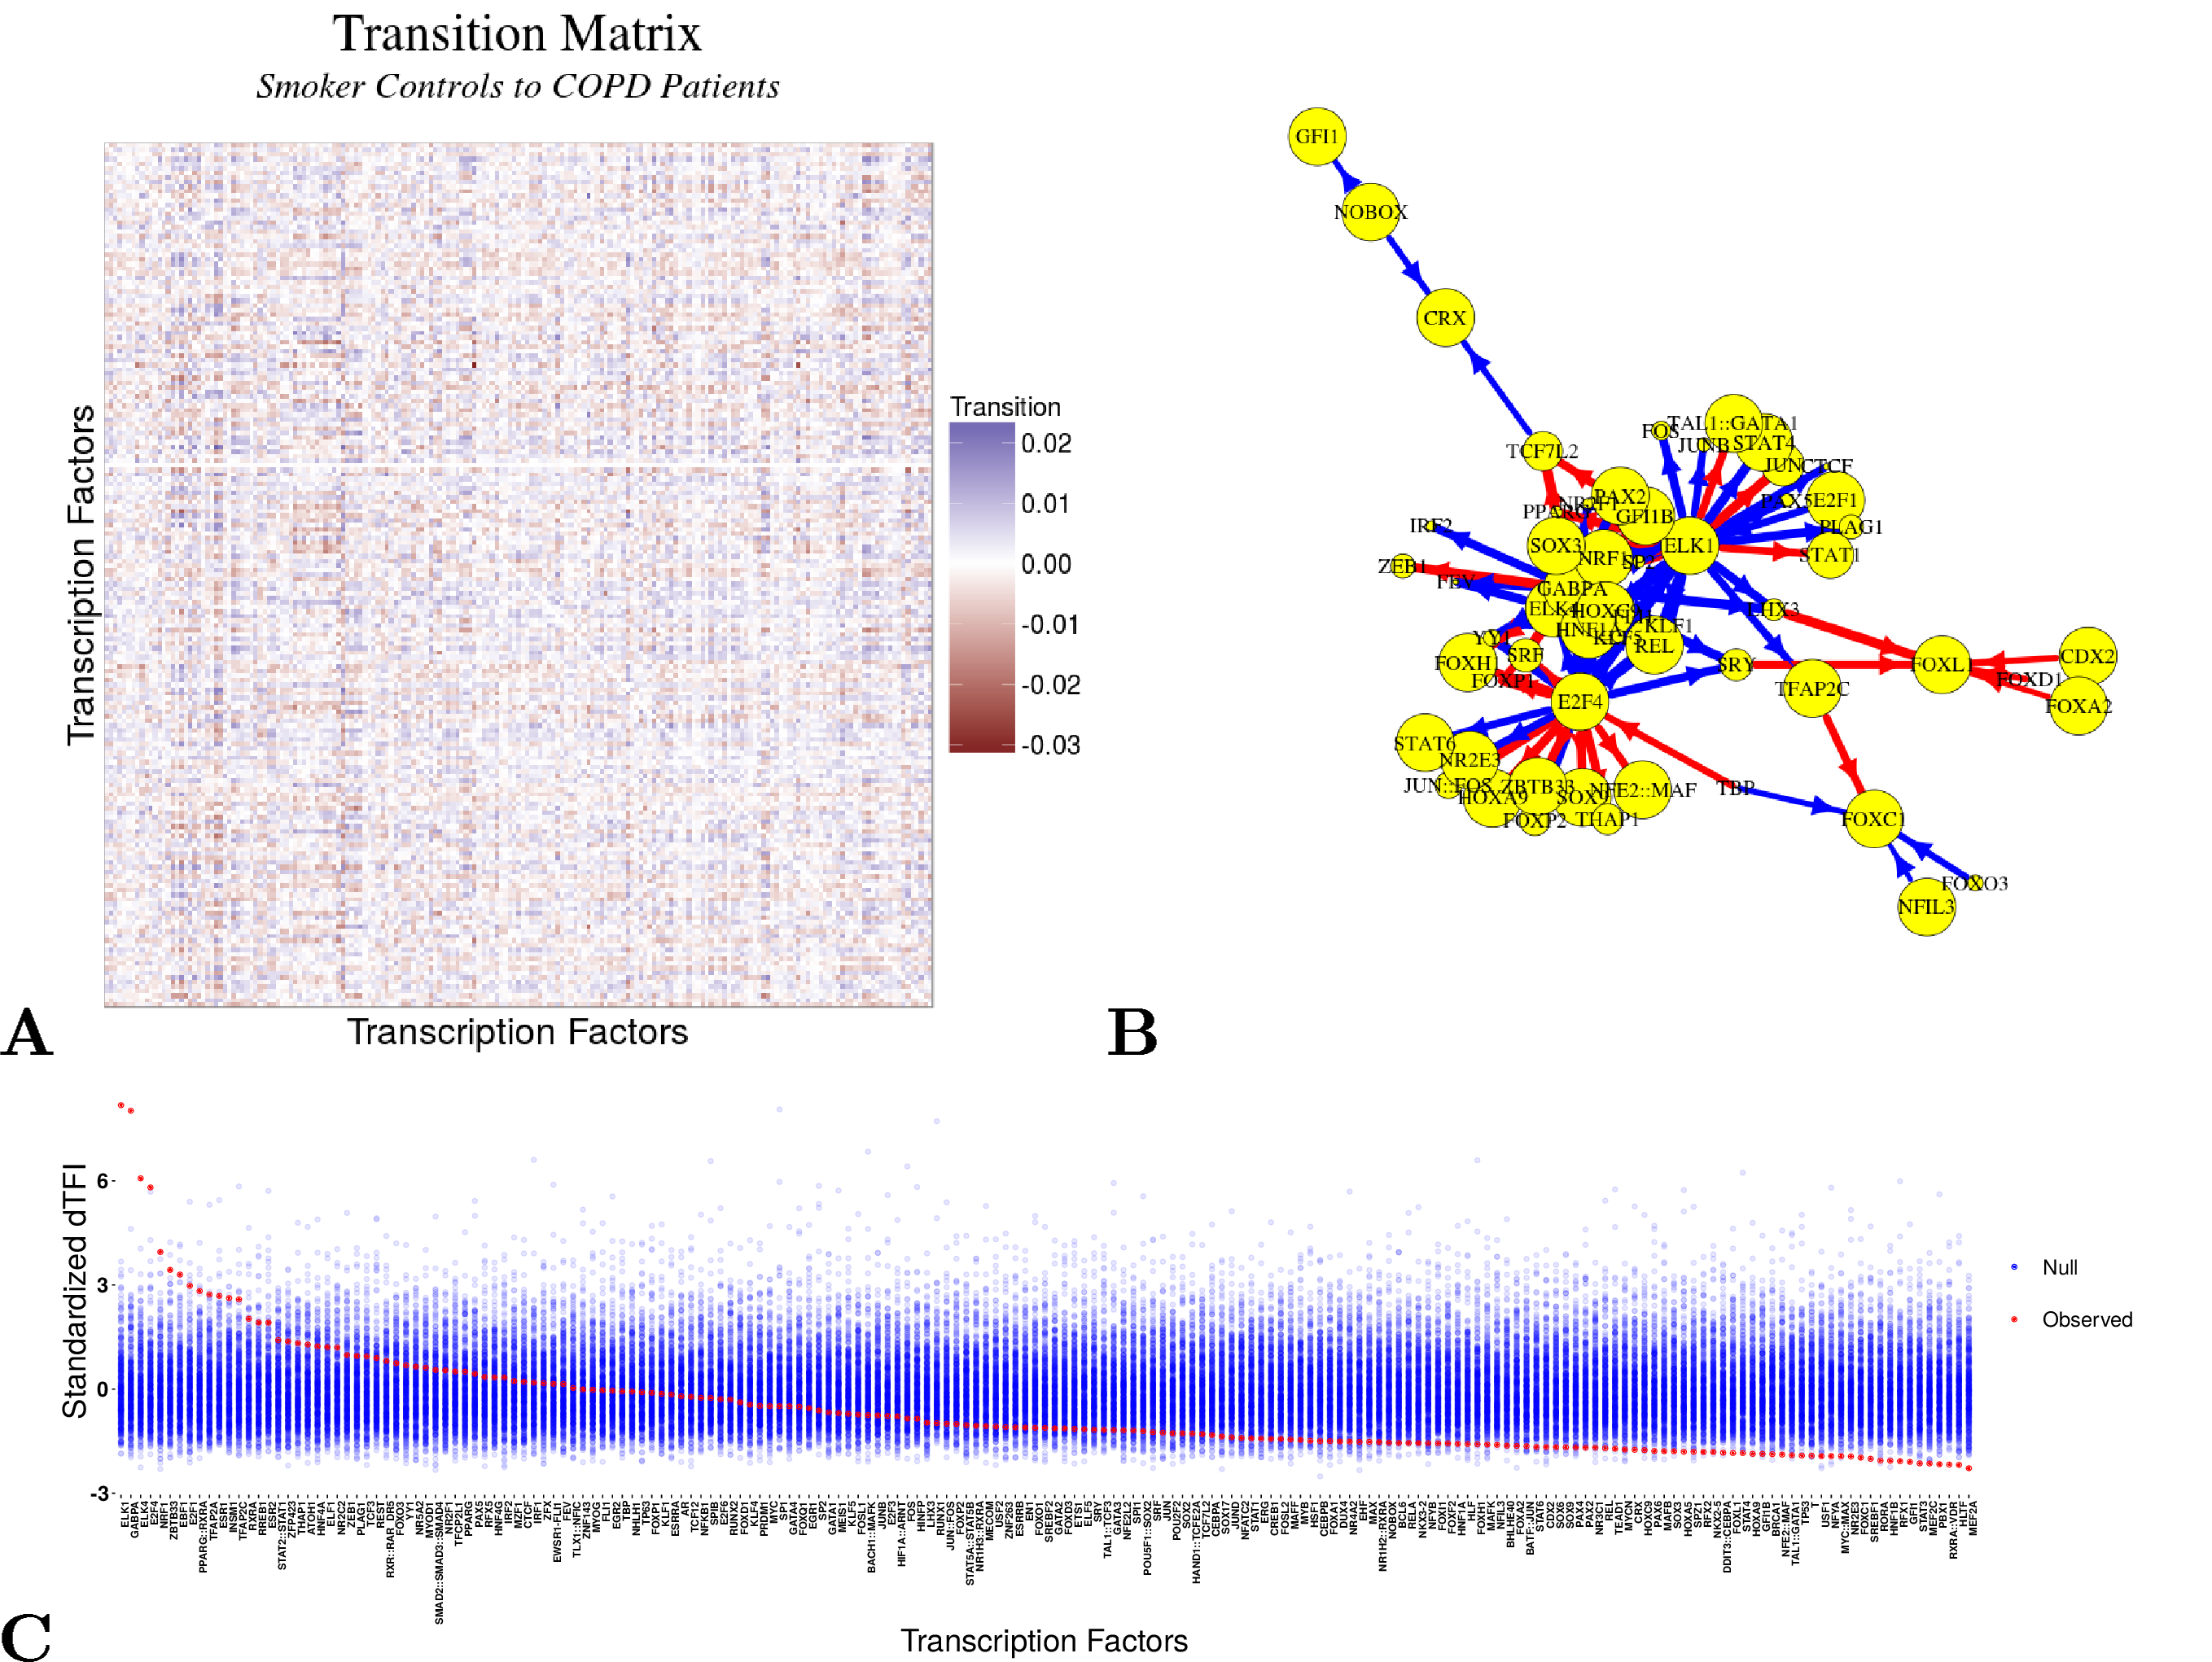
\includegraphics[width=0.49\columnwidth]{figures/figure2COPDGene}}}

\begin{raggedright}
\textbf{}\subfloat[\textbf{LGRC}]{\textbf{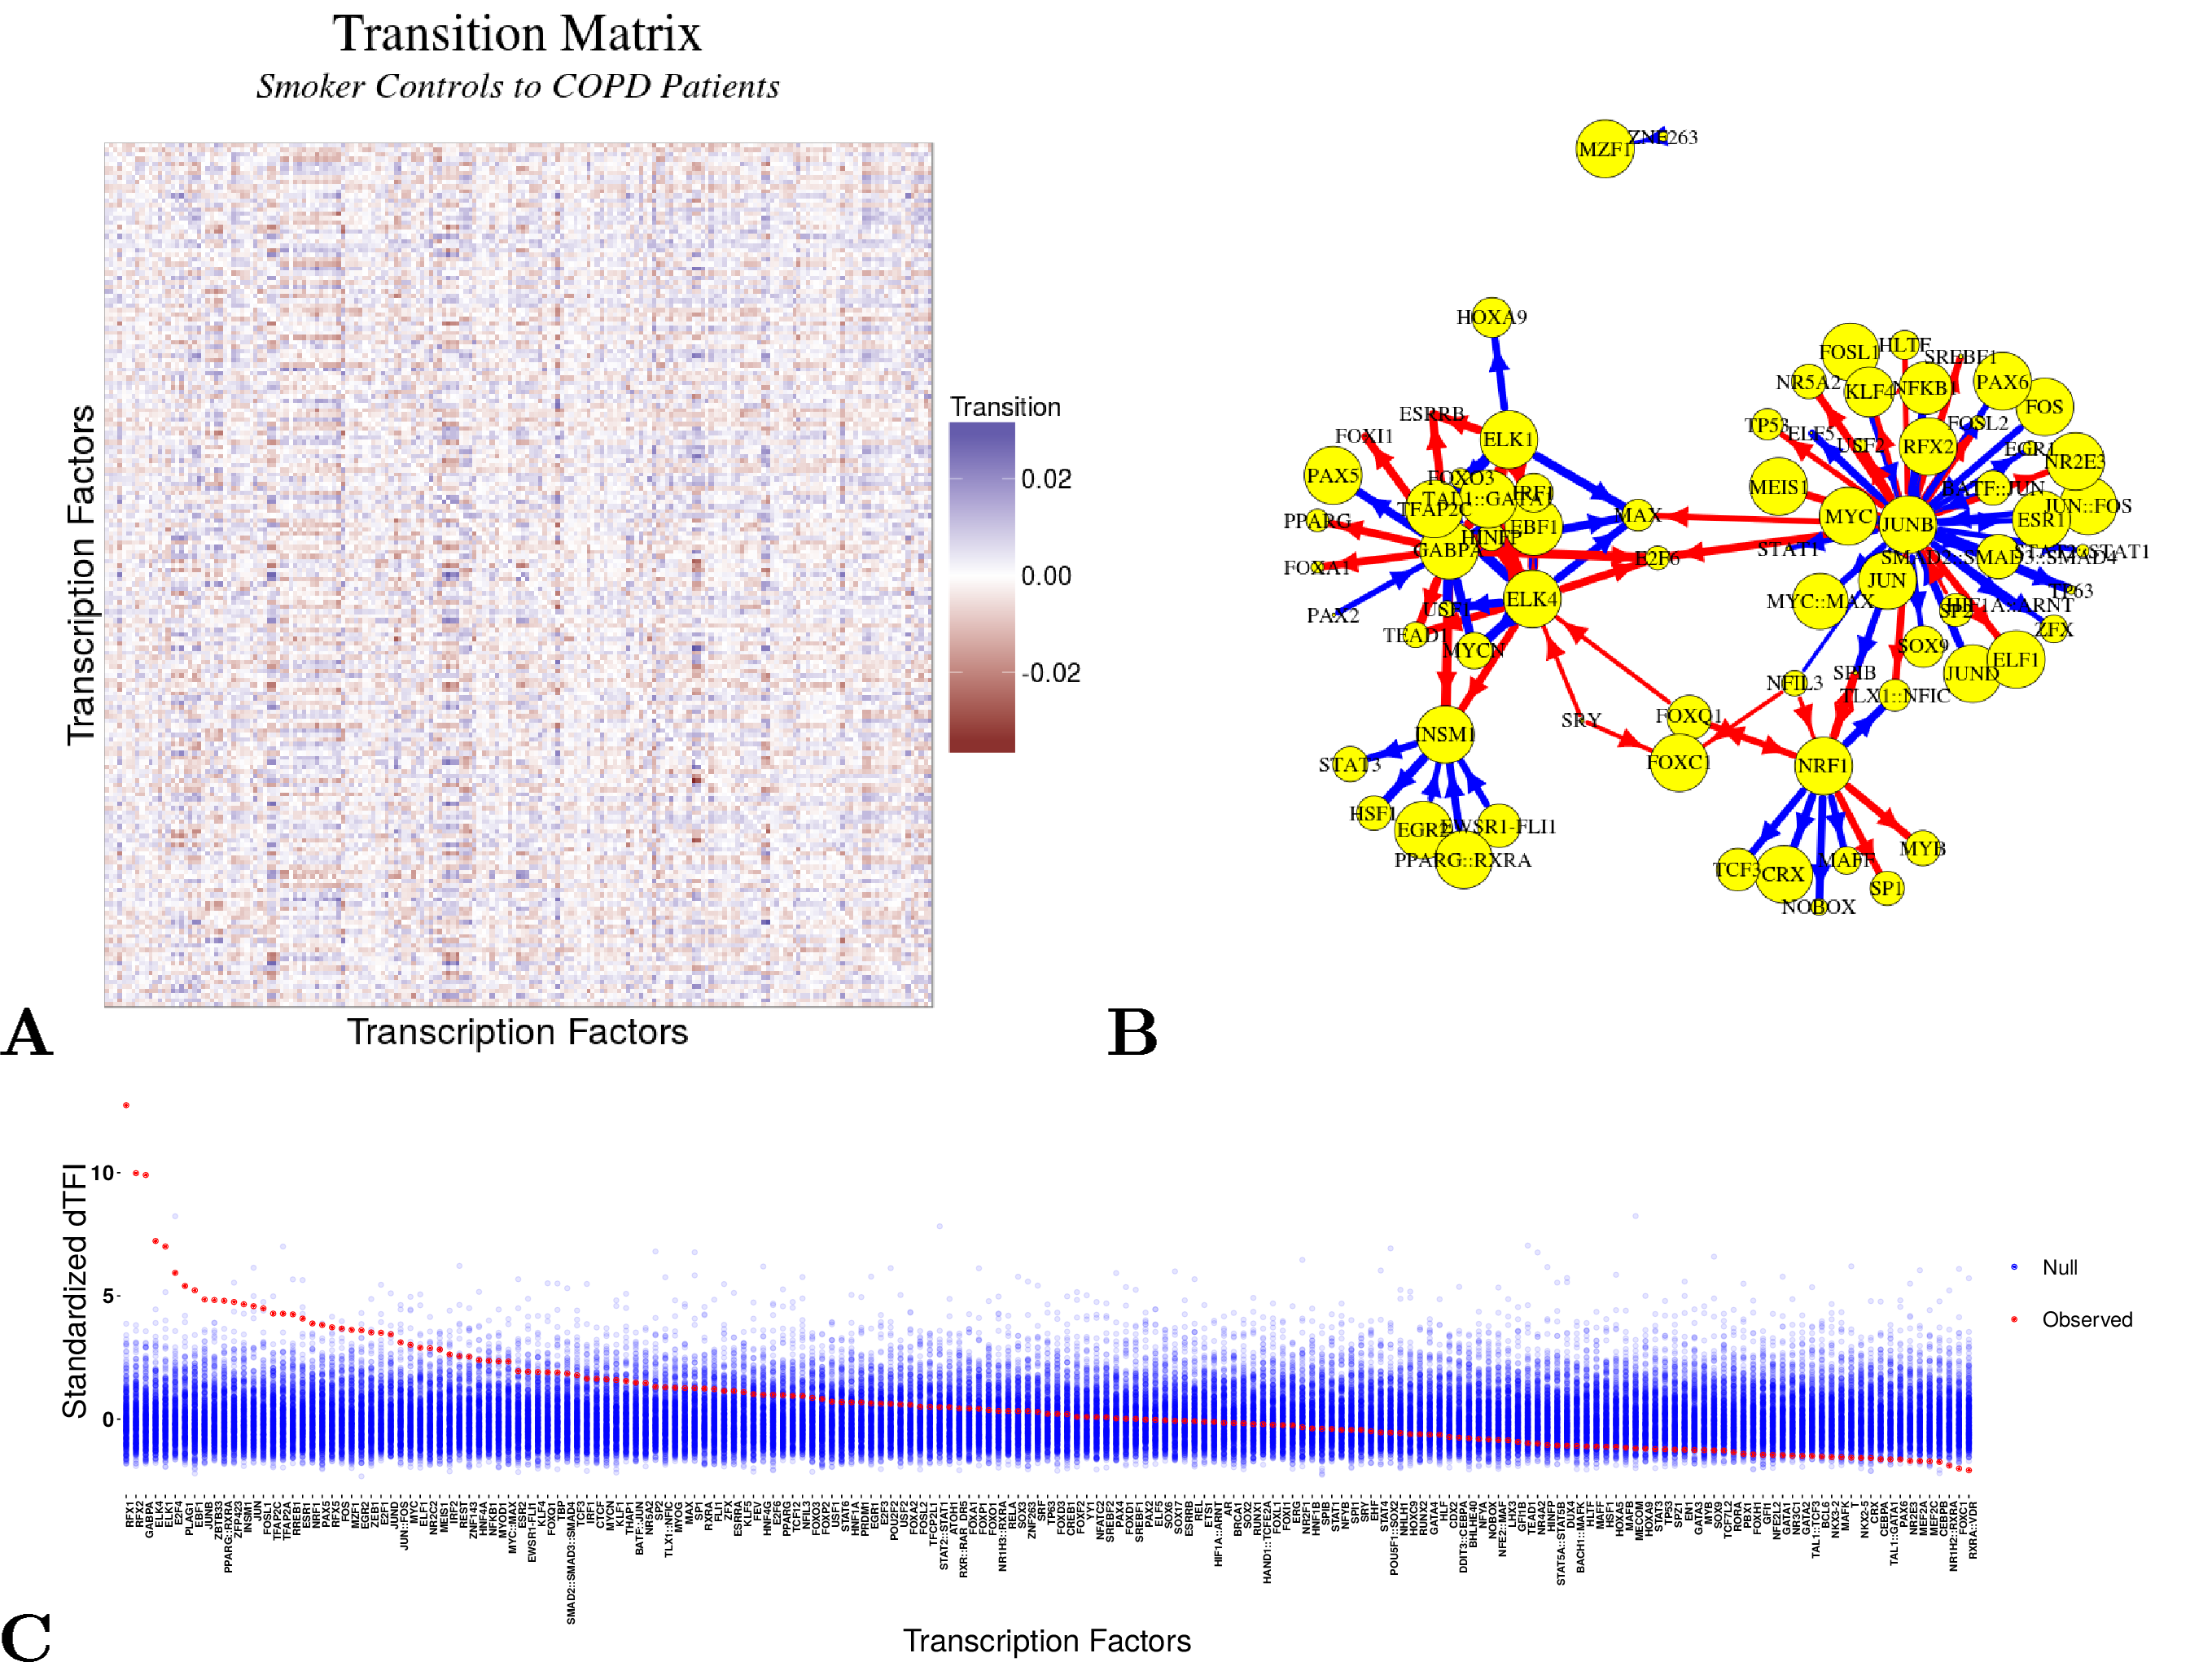
\includegraphics[width=0.49\columnwidth]{figures/figure2LGRC}}}
\par\end{raggedright}

\begin{raggedright}
\textbf{}\subfloat[\textbf{LTCOPD}]{\textbf{\includegraphics[width=0.49\columnwidth]{figures/figure2LTCOPD}}}
\par\end{raggedright}

\caption{\textbf{MONSTER analysis results for 4 studies (ECLIPSE reproduced
in main text) }See Figure 2 in main text for plot descriptions.}
\end{figure}


\begin{figure}
\textbf{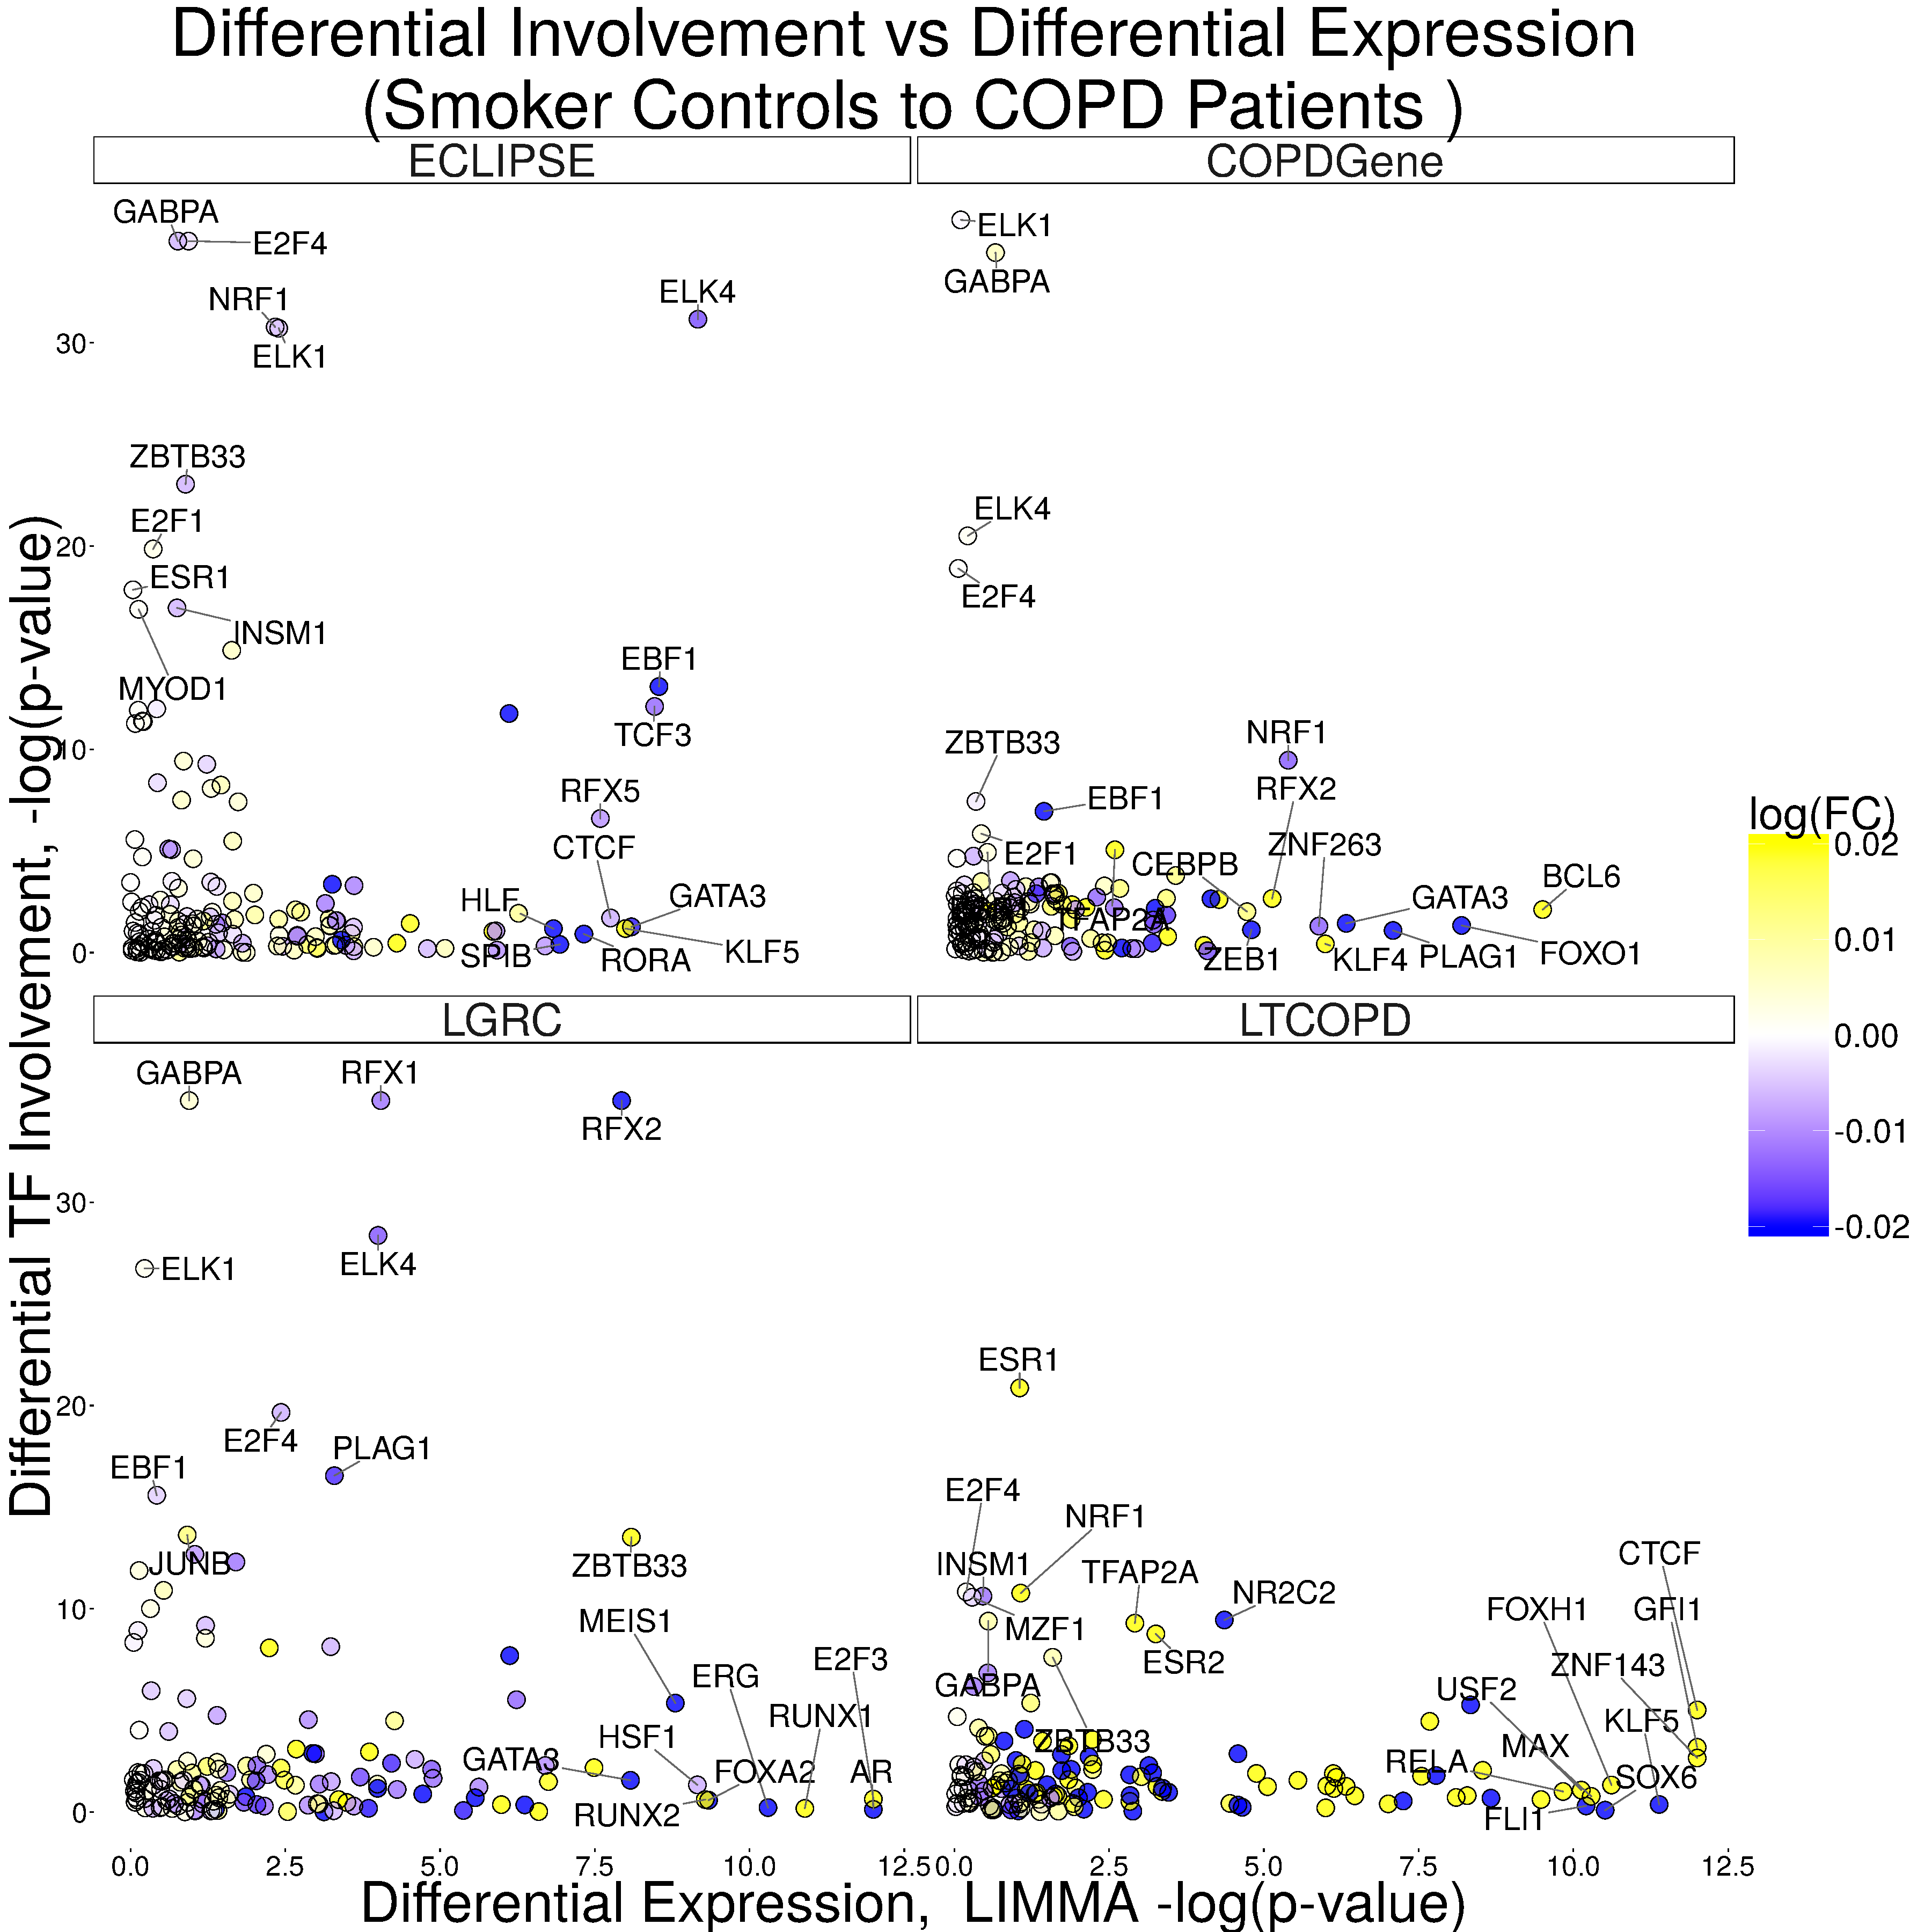
\includegraphics[width=1\columnwidth]{figures/dTFIvsLIMMAall}
}\caption{\textbf{Differentially transcription factor involvement vs differential
gene expression in four studies of COPD.} MONSTER commonly finds transcription
factors which are differentially involved but are expressed at similar
levels across cases and controls. Likewise, differential expression
does not indicate differential involvement in MONSTER. For those transcription
factors which are differentially involved, but not differentially
expressed, the change in involvement suggests behavioral alterations
at a post-transcriptional stage. Importantly, the results found in
this scenario could not have been identified using conventional differential
expression methods.}


\label{fig:sup_expression}
\end{figure}



\subsection*{\uline{Efficiency of estimation}}

Here we demonstrate that MONSTER is more efficient at estimating state
transitions than di

Let $\mathbf{x}_{p}$ be a Gaussian $p$-vector representing a sample
of gene expression data containing $q$ transcription factors and
$p-q$ non-transcription factor genes. 
\[
\mathbf{x}_{p}\sim N\left(\mathbf{\mu},\Sigma\right)
\]
where $\mathbf{\mu}$ is the $p$-vector of mean gene expression values
and $\Sigma$ is the $p\times p$ variance-covariance matrix. In this
scenario, $\Sigma$ may be regarded as a combination of two independent
variance-covariance sources- (1) biological signal, (2) biological
noise and technical noise.

In investigating gene regulation, many network inference methods are
constructed for the estimation of the $p\times q$ subset of $\Sigma$
pertaining to the effect of the $q$ TFs on the $p$ genes. In identifying
drivers of state transitions, we seek to focus on the $q\times q$
matrix of TF-TF effects. We show that our method vastly ourperforms
commonly used network inference methods in estimating these specific
effects.

Consider a state change between two experimental conditions, A and
B, characterized by an alteration of size $\delta$ to the biological
signal component of the TF-TF variance-covariance matrix at point
$\Sigma_{i,j}$ where $i$ and $j$ are indices for two TFs in $\Sigma$.

Using a univariate coexpression calculation (the basis for Pearson
networks and WGCNA estimates), the estimated variance of our estimate
of $\delta$ can be calculated:

\[
-\rho_{A}<\delta<\rho_{A},\delta+\rho_{A}\le1
\]


\begin{eqnarray*}
Var\left(\hat{\rho}_{i,j,A}-\hat{\rho}_{i,j,B}\right) & = & Var\left(\hat{\delta}_{cor}\right)\\
 &  & Var\left(\hat{\rho}_{i,j,A}\right)+Var\left(\hat{\rho}_{i,j,B}\right)\\
 & = & \frac{1-\rho_{i,j,A}^{2}}{n_{A}-2}+\frac{1-\rho_{i,j,B}^{2}}{n_{B}-2}\\
 & = & \frac{1}{n_{A}-2}+\frac{1}{n_{B}-2}-\frac{\rho_{i,j,A}^{2}}{n_{A}-2}-\frac{\rho_{i,j,B}^{2}}{n_{B}-2}
\end{eqnarray*}
Meanwhile, in condition B the new correlation of $TF_{i}$ with some
gene, $gene_{k}$ $k\in1,2\dots p$ , denoted $cor^{*}$, becomes
\[
cor^{*}\left(TF_{i},gene_{k}\right)=cor\left(TF_{i},gene_{k}\right)+\delta cor\left(TF_{j},gene_{k}\right)
\]
where the term $\delta cor\left(TF_{j},gene_{k}\right)$ is the change
due to the interaction of $TF_{i}$ and $TF_{j}$. 

The variance of our estimate using the transition matrix can be expressed
as follows:
\begin{eqnarray*}
Var\left(TM_{i,j}\right) & = & Var\left(\hat{\delta}_{TM}\right)\\
 & = & \frac{\left(\frac{1}{p}\right)\sum_{k=1}^{p}vVar\left(\hat{\rho}_{i,k,A}-\hat{\rho}_{i,k,B}\right)}{\sum_{k=1}^{p}\left(\rho_{j,k}-\bar{\rho_{j}}\right)^{2}}\\
\\
 & = & \frac{\left(\frac{1}{p}\right)\sum_{k=1}^{p}\left[Var\left(\hat{\rho}_{i,k,A}\right)+Var\left(\hat{\rho}_{i,k,B}\right)\right]}{\sum_{k=1}^{p}\left(\rho_{j,k}-\bar{\rho_{i}}\right)^{2}}\\
 & \le & \frac{\left(\frac{1}{p}\right)\sum_{k=1}^{p}\left[\frac{1}{n_{A}-2}+\frac{1}{n_{B}-2}\right]}{\sum_{k=1}^{p}\left(\rho_{j,k}-\bar{\rho_{i}}\right)^{2}}\\
 & \le & \frac{\frac{1}{n_{A}-2}+\frac{1}{n_{B}-2}}{\sum_{k=1}^{p}\left(\rho_{j,k}-\bar{\rho_{i}}\right)^{2}}\\
 & \le & \frac{Var\left(\hat{\delta}_{cor}\right)+\frac{\rho_{i,j,A}^{2}}{n_{A}-2}+\frac{\rho_{i,j,B}^{2}}{n_{B}-2}}{\sum_{k=1}^{p}\left(\rho_{j,k}-\bar{\rho_{i}}\right)^{2}}\\
 & \le & Var\left(\hat{\delta}_{cor}\right)+\frac{Var\left(\hat{\delta}_{cor}\right)\left(1-\sum_{k=1}^{p}\left(\rho_{j,k}-\bar{\rho_{i}}\right)^{2}\right)+\frac{\rho_{i,j,A}^{2}}{n_{A}-2}+\frac{\rho_{i,j,B}^{2}}{n_{B}-2}}{\sum_{k=1}^{p}\left(\rho_{j,k}-\bar{\rho_{i}}\right)^{2}}
\end{eqnarray*}
So we have that $Var\left(TM_{i,j}\right)<Var\left(\hat{\delta}_{cor}\right)$
when
\[
Var\left(\hat{\delta}_{cor}\right)\left(1-\sum_{k=1}^{p}\left(\rho_{j,k}-\bar{\rho_{i}}\right)^{2}\right)<\frac{\rho_{i,j,A}^{2}}{n_{A}-2}+\frac{\rho_{i,j,B}^{2}}{n_{B}-2}
\]
Since each term except $\left(1-\sum_{k=1}^{p}\left(\rho_{j,k}-\bar{\rho_{i}}\right)^{2}\right)$
is strictly non-negative, we see that this inequality holds when 
\[
\sum_{k=1}^{p}\left(\rho_{j,k}-\bar{\rho_{i}}\right)^{2}<1
\]
Thus, we have a more efficient estimator of $\delta$ when 
\[
p>\frac{1}{Var\left(\rho_{j,k}\right)}
\]
In practice, we typically have a large number of genes, $p$, so that
our transition matrix estimator will be expected to be dramatically
more efficient than the commonly used Pearson or WGCNA estimators
for estimating transcription factor- transcription factor interactions.

\begin{table}
\textbf{A} Top significantly differentially involved transcription
factors

{\center {\tiny

\begin{tabular}{|c||c|c|c||c|c|c||c|c|c||c|c|c|}
\cline{2-13} 
\multicolumn{1}{c|}{} & \multicolumn{3}{c||}{ECLIPSE} & \multicolumn{3}{c||}{COPDGene} & \multicolumn{3}{c||}{LGRC} & \multicolumn{3}{c|}{LTCOPD}\tabularnewline
\hline 
TF & dTFI & rank & FDR & dTFI & rank & FDR & dTFI & rank & FDR & dTFI & rank & FDR\tabularnewline
\hline 
\hline 
SP2 & .0314 &  1 & .0357 & .0100 &  9 & .6812 & .0213 &  6 & .3752 & .0176 &  2 & .7438\tabularnewline
\hline 
E2F4 & .0236 &  2 & <.0001 & .0143 &  3 & <.0001 & .0160 & 14 & .037 & .0148 &  7 & <.0001\tabularnewline
\hline 
SP1 & .0230 &  3 & .1551 & .0089 &  18 & .7721 & .0179 & 10 & .3594 & .0169 &  4 & .5516\tabularnewline
\hline 
ZNF263 & .0226 &  4 & .311 & .0089 &  16 & .3372 & .0177 & 11 & .7716 & .0152 &  6 & .927\tabularnewline
\hline 
EGR1 & .0224 &  5 & .1242 & .0079 &  23 & .7597 & .0124 & 28 & .6892 & .0152 &  5 & .5305\tabularnewline
\hline 
NRF1 & .0196 &  6 & <.0001 & .0115 &  5 & .0304 & .0122 & 30 & <.0001 & .0139 & 11 & .0558\tabularnewline
\hline 
GABPA & .0185 &  7 & <.0001 & .0157 &  2 & <.0001 & .0176 & 12 & <.0001 & .0097 & 32 & .0853\tabularnewline
\hline 
ELK1 & .0177 &  8 & <.0001 & .0174 &  1 & <.0001 & .0151 & 17 & <.0001 & .0083 & 40 & .2099\tabularnewline
\hline 
ZFX & .0175 &  9 & <.0001 & .0076 &  24 & .8366 & .0103 & 40 & .4348 & .0132 & 16 & .2739\tabularnewline
\hline 
KLF4 & .0173 &  10 & .1025 & .0072 &  28 & .8142 & .0143 & 21 & .2312 & .0119 & 20 & .5516\tabularnewline
\hline 
ESR1 & .0169 &  11 & .0357 & .0106 &  7 & .0941 & .0127 & 27 & .0888 & .0176 &  3 & <.0001\tabularnewline
\hline 
ELK4 & .0168 &  12 & <.0001 & .0125 &  4 & <.0001 & .0152 & 16 & <.0001 & .0086 & 39 & .1318\tabularnewline
\hline 
TFAP2C & .0139 &  17 & .0656 & .0114 &  6 & .0941 & .0148 & 19 & .037 & .0121 & 19 & .2099\tabularnewline
\hline 
PLAG1 & .0124 &  21 & .263 & .0092 &  15 & .4136 & .0219 &  5 & <.0001 & .0146 &  8 & .1554\tabularnewline
\hline 
FOXQ1 & .0115 &  28 & .9318 & .0099 &  10 & .7905 & .0209 &  7 & .2846 & .0107 & 27 & .927\tabularnewline
\hline 
FOSL1 & .0082 &  57 & .9175 & .0061 &  41 & .6166 & .0220 &  4 & .037 & .0131 & 17 & .3496\tabularnewline
\hline 
NFIL3 & .0077 &  62 & .2365 & .0067 &  33 & .0304 & .0264 &  1 & .4669 & .0209 &  1 & .7121\tabularnewline
\hline 
FOS & .0068 &  73 & .9175 & .0057 &  48 & .5212 & .0198 &  9 & .037 & .0112 & 24 & .5139\tabularnewline
\hline 
JUNB & .0067 &  77 & .9318 & .0059 &  43 & .6392 & .0236 &  2 & <.0001 & .0146 &  9 & .2299\tabularnewline
\hline 
RFX1 & .0019 & 159 & .3532 & .0009 & 164 & <.0001 & .0233 &  3 & <.0001 & .0070 & 48 & .3496\tabularnewline
\hline 
RFX2 & .0019 & 158 & .4041 & .0012 & 163 & .0482 & .0200 &  8 & <.0001 & .0049 & 81 & .6245\tabularnewline
\hline 
\end{tabular}}}

\textbf{B} Differential gene expression for significantly involved
transcription factors.

{\center {\tiny

\begin{tabular}{|c||c|c||c|c||c|c||c|c|}
\cline{2-9} 
\multicolumn{1}{c|}{} & \multicolumn{2}{c||}{ECLIPSE} & \multicolumn{2}{c||}{COPDGene} & \multicolumn{2}{c||}{LGRC} & \multicolumn{2}{c|}{LTCOPD}\tabularnewline
\hline 
TF & dTFI rank & LIMMA p & dTFI rank & LIMMA p & dTFI rank & LIMMA p & dTFI rank & LIMMA p\tabularnewline
\hline 
\hline 
SP2 &  1 & .1756 &  9 & .6517 &  6 & .0075 &  2 & .0009\tabularnewline
\hline 
E2F4 &  2 & .3913 &  3 & .9367 & 14 & .0878 &  7 & .8232\tabularnewline
\hline 
SP1 &  3 & .3634 &  18 & .0838 & 10 & .4242 &  4 & .9759\tabularnewline
\hline 
ZNF263 &  4 & .9834 &  16 & .0028 & 11 & .0271 &  6 & .1859\tabularnewline
\hline 
EGR1 &  5 & .4379 &  23 & .8540 & 28 & .7979 &  5 & .0378\tabularnewline
\hline 
NRF1 &  6 & .0966 &  5 & .0045 & 30 & .2974 & 11 & .3418\tabularnewline
\hline 
GABPA &  7 & .4650 &  2 & .5138 & 12 & .3868 & 32 & .5771\tabularnewline
\hline 
ELK1 &  8 & .0913 &  1 & .9010 & 17 & .7968 & 40 & .0005\tabularnewline
\hline 
ZFX &  9 & .8253 &  24 & .5795 & 40 & .0474 & 16 & .1572\tabularnewline
\hline 
KLF4 &  10 & .1915 &  28 & .0025 & 21 & .0526 & 20 & .1159\tabularnewline
\hline 
ESR1 &  11 & .9598 &  7 & .5853 & 27 & .7246 &  3 & .3477\tabularnewline
\hline 
ELK4 &  12 & .0001 &  4 & .8057 & 16 & .0183 & 39 & .7314\tabularnewline
\hline 
TFAP2C &  17 & .2318 &  6 & .9574 & 19 & .5853 & 19 & .6754\tabularnewline
\hline 
PLAG1 &  21 & .0384 &  15 & .0008 &  5 & .0371 &  8 & .9523\tabularnewline
\hline 
FOXQ1 &  28 & .4543 &  10 & .5314 &  7 & .0503 & 27 & .5340\tabularnewline
\hline 
FOSL1 &  57 & .5850 &  41 & .6995 &  4 & .8708 & 17 & .3686\tabularnewline
\hline 
NFIL3 &  62 & .0404 &  33 & .1191 &  1 & .7605 &  1 & .8650\tabularnewline
\hline 
FOS &  73 & .5156 &  48 & .6668 &  9 & .9500 & 24 & .7891\tabularnewline
\hline 
JUNB &  77 & .0197 &  43 & .9526 &  2 & .3996 &  9 & .6077\tabularnewline
\hline 
RFX1 & 159 & .0361 & 164 & .0885 &  3 & .0175 & 48 & .8285\tabularnewline
\hline 
RFX2 & 158 & .0109 & 163 & .0059 &  8 & .0004 & 81 & .1345\tabularnewline
\hline 
\end{tabular}}}\caption{\textbf{Top Transcription Factor Hits.} \textbf{A} Combined list of
TFs which were among the top 10 hits (out of 166 available TFs) in
any of the 4 studies, ordered by the dTFI in the ECLIPSE study. For
each study, columns indicate the TF's (1) differential TF Involvement,
(2) dTFI Rank within list of TFs, (3) and Significance of dTFI by
false discovery rate. \textbf{B} The same list of top transcription
factors evaluated for differential gene expression with p-value for
differential gene expression analysis using LIMMA~\cite{ritchie2015limma}.
Notably, a substantial number of differentially involved transcription
factors do not exhibit gene expression differentiation, highlighting
the ability of MONSTER to identify key features distinguising phenotypes
which are not detectable via gene expression analysis.}
\end{table}


\bibliographystyle{plain}
\bibliography{dissertation_research}

\end{document}
